\documentclass[10pt]{beamer}

% Use this to only show the final state of the frames
%\documentclass[handout,10pt]{beamer}

% %%%%%%%%%%%%%%%%%%%%%%%%%%%%%%%%%%%%%%%%%%%%%%%%%%%%%%%%%%%%%%%%%%%%%%%%%%%%%%
% \embedvideo{<poster or text>}{<video file (MP4+H264)>}
% \embedvideo*{...}{...}                     % auto-play
%%%%%%%%%%%%%%%%%%%%%%%%%%%%%%%%%%%%%%%%%%%%%%%%%%%%%%%%%%%%%%%%%%%%%%%%%%%%%%

\usepackage[bigfiles]{pdfbase}
\ExplSyntaxOn
\NewDocumentCommand\embedvideo{smm}{
  \group_begin:
  \leavevmode
  \tl_if_exist:cTF{file_\file_mdfive_hash:n{#3}}{
    \tl_set_eq:Nc\video{file_\file_mdfive_hash:n{#3}}
  }{
    \IfFileExists{#3}{}{\GenericError{}{File~`#3'~not~found}{}{}}
    \pbs_pdfobj:nnn{}{fstream}{{}{#3}}
    \pbs_pdfobj:nnn{}{dict}{
      /Type/Filespec/F~(#3)/UF~(#3)
      /EF~<</F~\pbs_pdflastobj:>>
    }
    \tl_set:Nx\video{\pbs_pdflastobj:}
    \tl_gset_eq:cN{file_\file_mdfive_hash:n{#3}}\video
  }
  %
  \pbs_pdfobj:nnn{}{dict}{
    /Type/RichMediaInstance/Subtype/Video
    /Asset~\video
    /Params~<</FlashVars (
      source=#3&
      skin=SkinOverAllNoFullNoCaption.swf&
      skinAutoHide=true&
      skinBackgroundColor=0x5F5F5F&
      skinBackgroundAlpha=0
    )>>
  }
  %
  \pbs_pdfobj:nnn{}{dict}{
    /Type/RichMediaConfiguration/Subtype/Video
    /Instances~[\pbs_pdflastobj:]
  }
  %
  \pbs_pdfobj:nnn{}{dict}{
    /Type/RichMediaContent
    /Assets~<<
      /Names~[(#3)~\video]
    >>
    /Configurations~[\pbs_pdflastobj:]
  }
  \tl_set:Nx\rmcontent{\pbs_pdflastobj:}
  %
  \pbs_pdfobj:nnn{}{dict}{
    /Activation~<<
      /Condition/\IfBooleanTF{#1}{PV}{XA}
      /Presentation~<</Style/Embedded>>
    >>
    /Deactivation~<</Condition/PI>>
  }
  %
  \hbox_set:Nn\l_tmpa_box{#2}
  \tl_set:Nx\l_box_wd_tl{\dim_use:N\box_wd:N\l_tmpa_box}
  \tl_set:Nx\l_box_ht_tl{\dim_use:N\box_ht:N\l_tmpa_box}
  \tl_set:Nx\l_box_dp_tl{\dim_use:N\box_dp:N\l_tmpa_box}
  \pbs_pdfxform:nnnnn{1}{1}{}{}{\l_tmpa_box}
  %
  \pbs_pdfannot:nnnn{\l_box_wd_tl}{\l_box_ht_tl}{\l_box_dp_tl}{
    /Subtype/RichMedia
    /BS~<</W~0/S/S>>
    /Contents~(embedded~video~file:#3)
    /NM~(rma:#3)
    /AP~<</N~\pbs_pdflastxform:>>
    /RichMediaSettings~\pbs_pdflastobj:
    /RichMediaContent~\rmcontent
  }
  \phantom{#2}
  \group_end:
}
\ExplSyntaxOff
%%%%%%%%%%%%%%%%%%%%%%%%%%%%%%%%%%%%%%%%%%%%%%%%%%%%%%%%%%%%%%%%%%%%%%%%%%%%%%

\usetheme[progressbar=frametitle]{metropolis}
\usepackage{appendixnumberbeamer}

\usepackage{booktabs}
%\usepackage[scale=2]{ccicons}

\usepackage{pgfplots}
\usepgfplotslibrary{dateplot}

%\usepackage[ruled,vlined]{algorithm2e}
\usepackage{amssymb}
\usepackage{gensymb}
\usepackage{xspace}
\usepackage{graphicx}
\usepackage{amsmath}
\newcommand{\themename}{\textbf{\textsc{metropolis}}\xspace}
\newcommand\restr[2]{\ensuremath{\left.#1\right|_{#2}}}

\usepackage{url}

\newcounter{TheoremCounter}
\resetcounteronoverlays{algocf}
\resetcounteronoverlays{TheoremCounter}

\title{Lovász-Stein Theorem}
\subtitle{Seminar Extremal Graph Theory}
\date{20.12.2021}
\institute{Advisors: \newline Prof. Dr. Maria Axenovich \& Dr. Alexander Neal Riasanovsky}
\author{Robin Link}


\begin{document}

\maketitle

\section{Lovász-Stein Theorem}
%\begin{frame}[fragile]{Motivation}
%    \centering{
%        \embedvideo*{
\includegraphics[height=.7\textheight]{Animations/SquareToCirclePreview}}{Animations/SquareToCircle.mp4}
%    }
%\end{frame}


\begin{frame}[fragile]{Motivation}
    \hspace*{-.25em}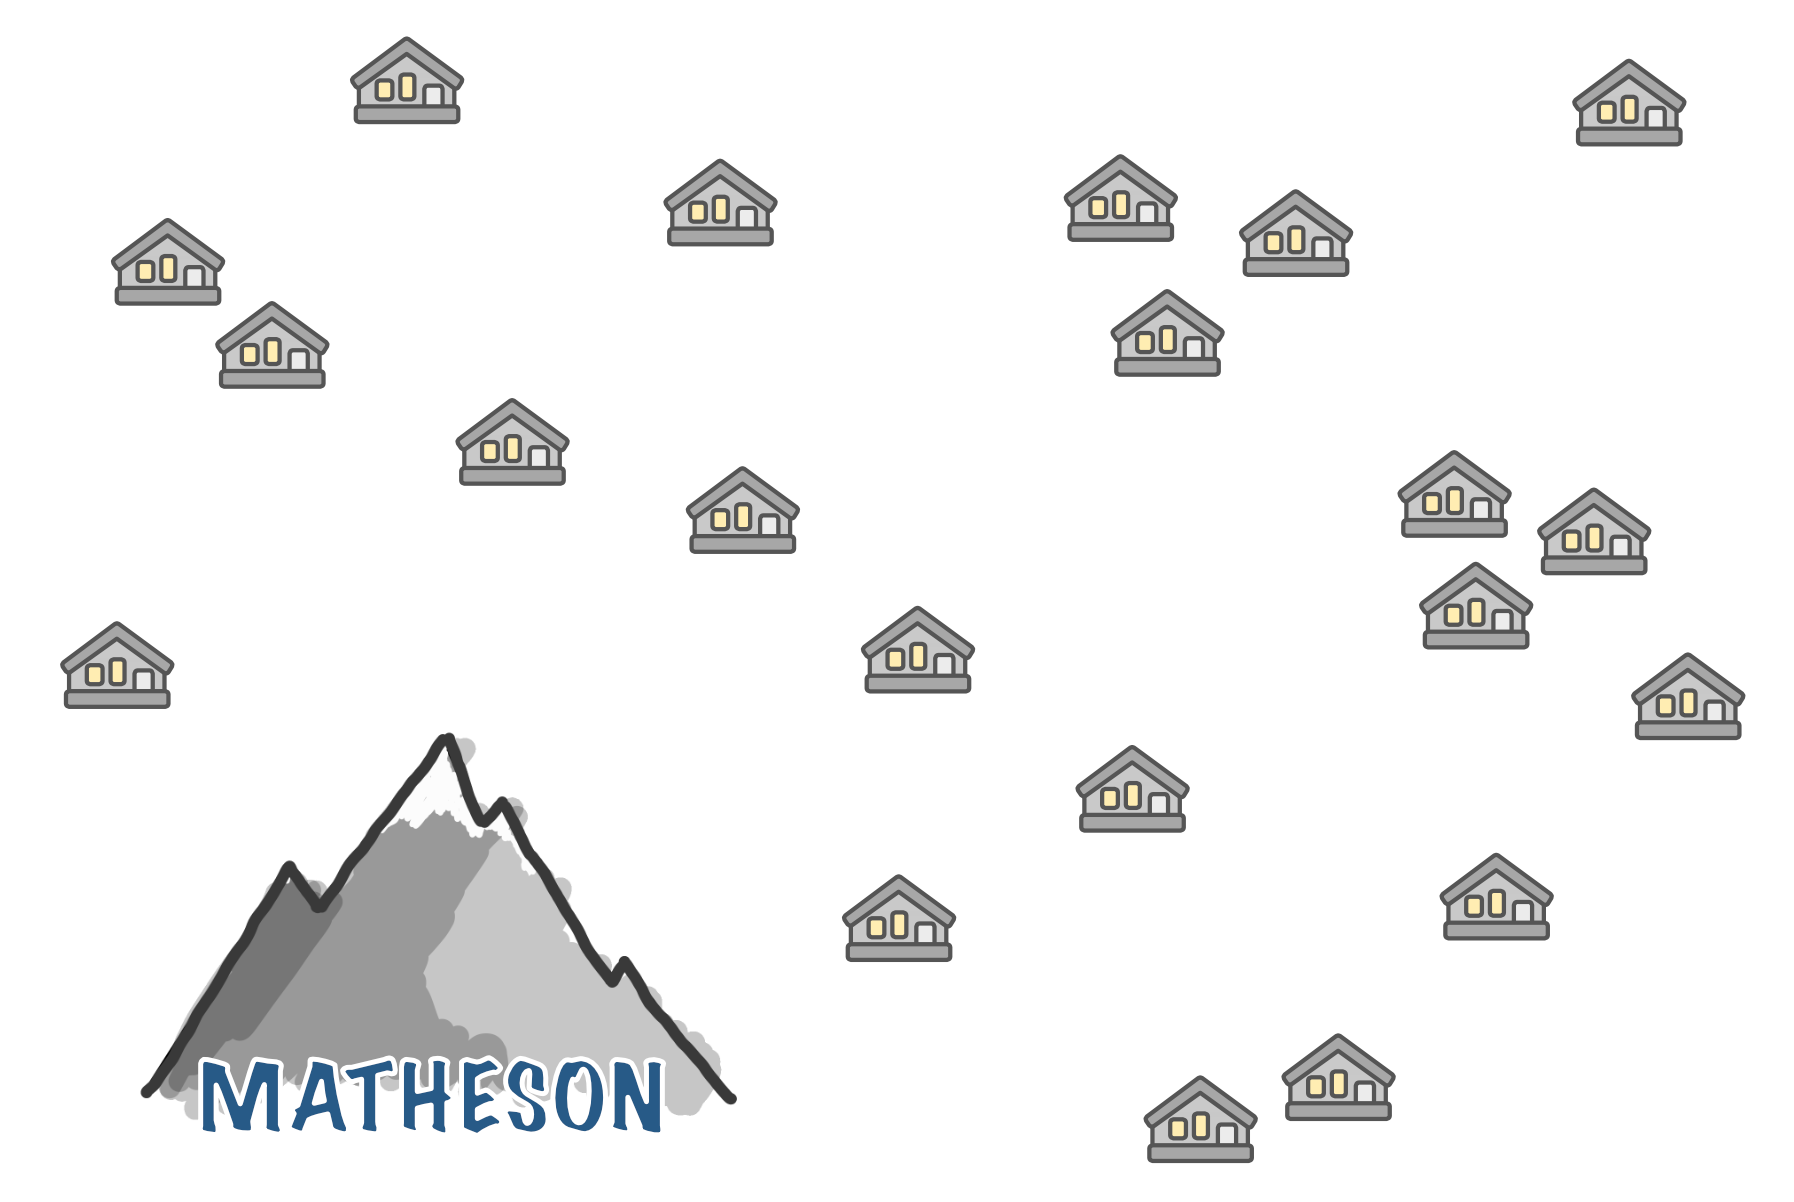
\includegraphics[width=\textwidth]{Images/Matheson/Matheson_01}
\end{frame}

\begin{frame}[fragile]{Motivation}
    \hspace*{-.25em}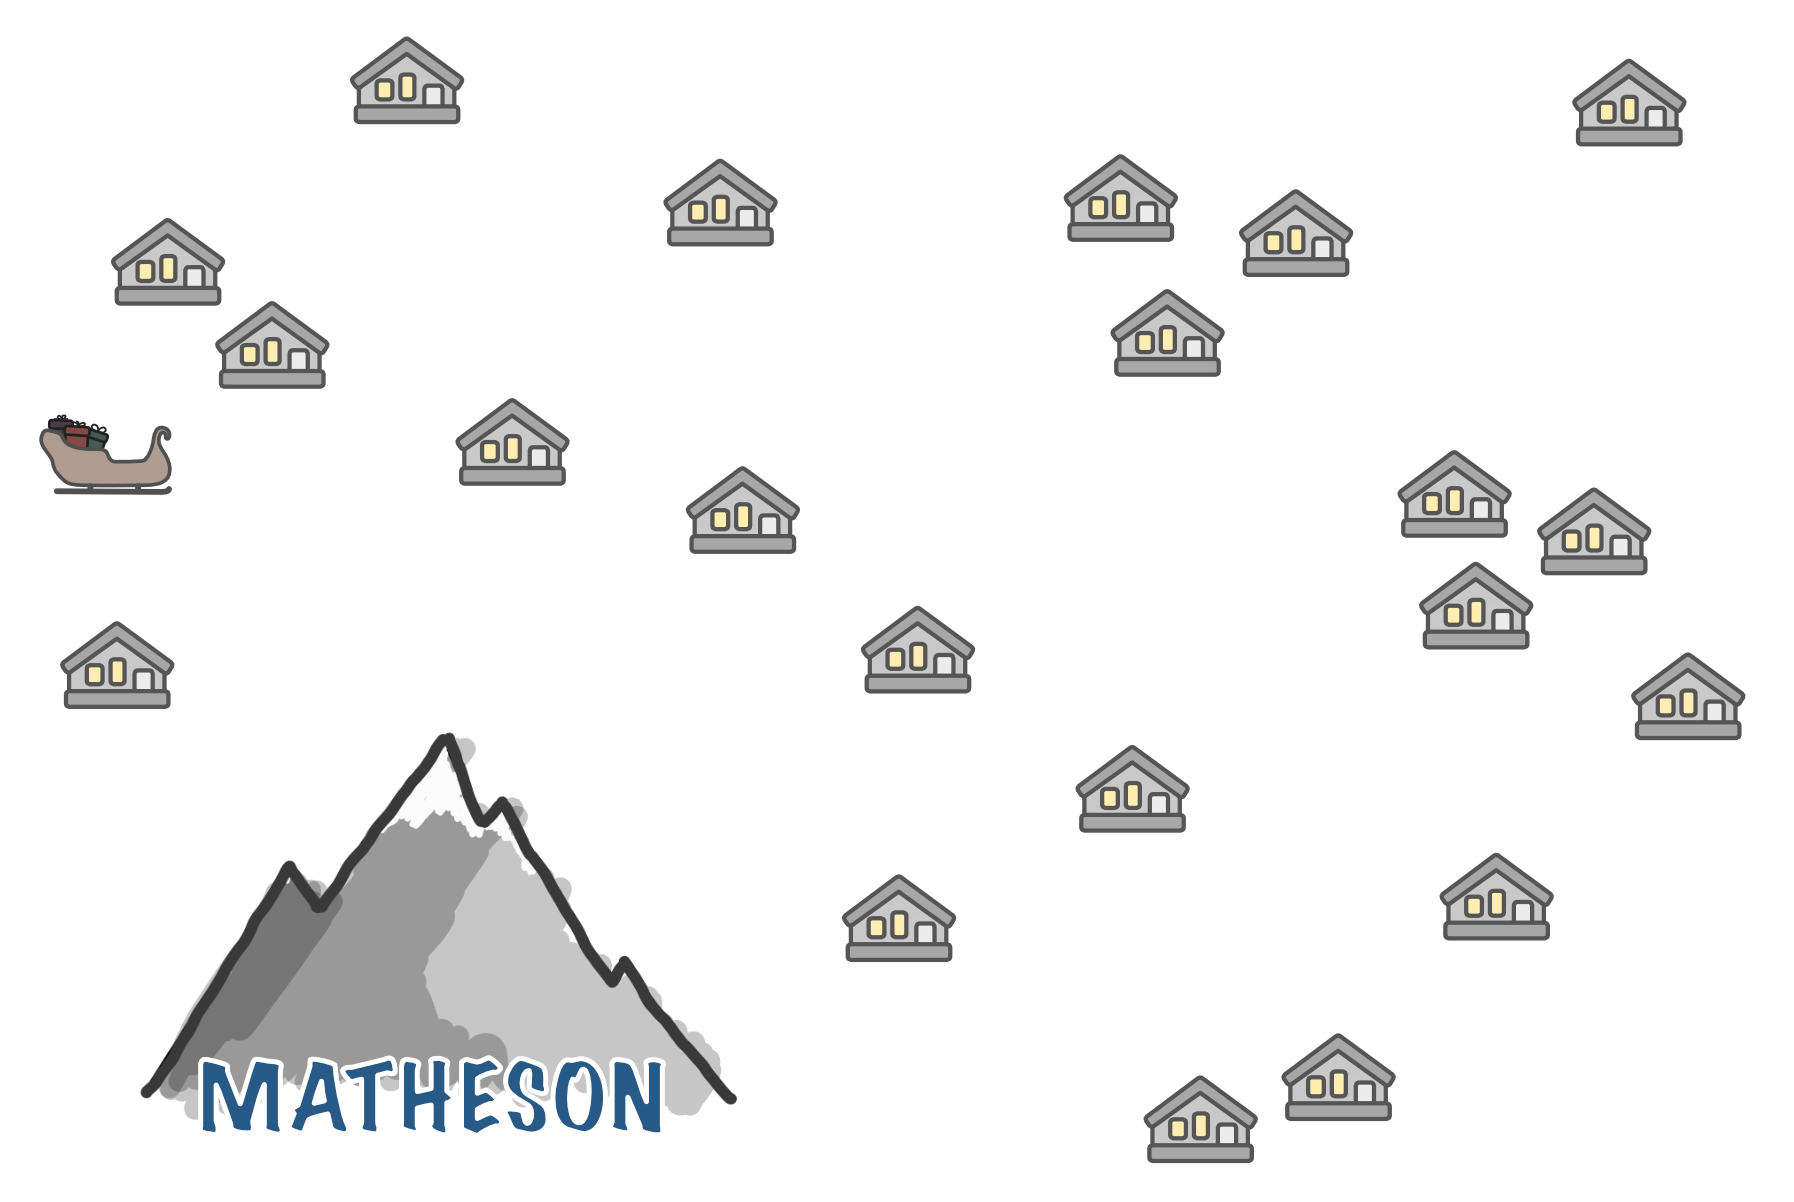
\includegraphics[width=\textwidth]{Images/Matheson/Matheson_02}
\end{frame}

\begin{frame}[fragile]{Motivation}
    \hspace*{-.25em}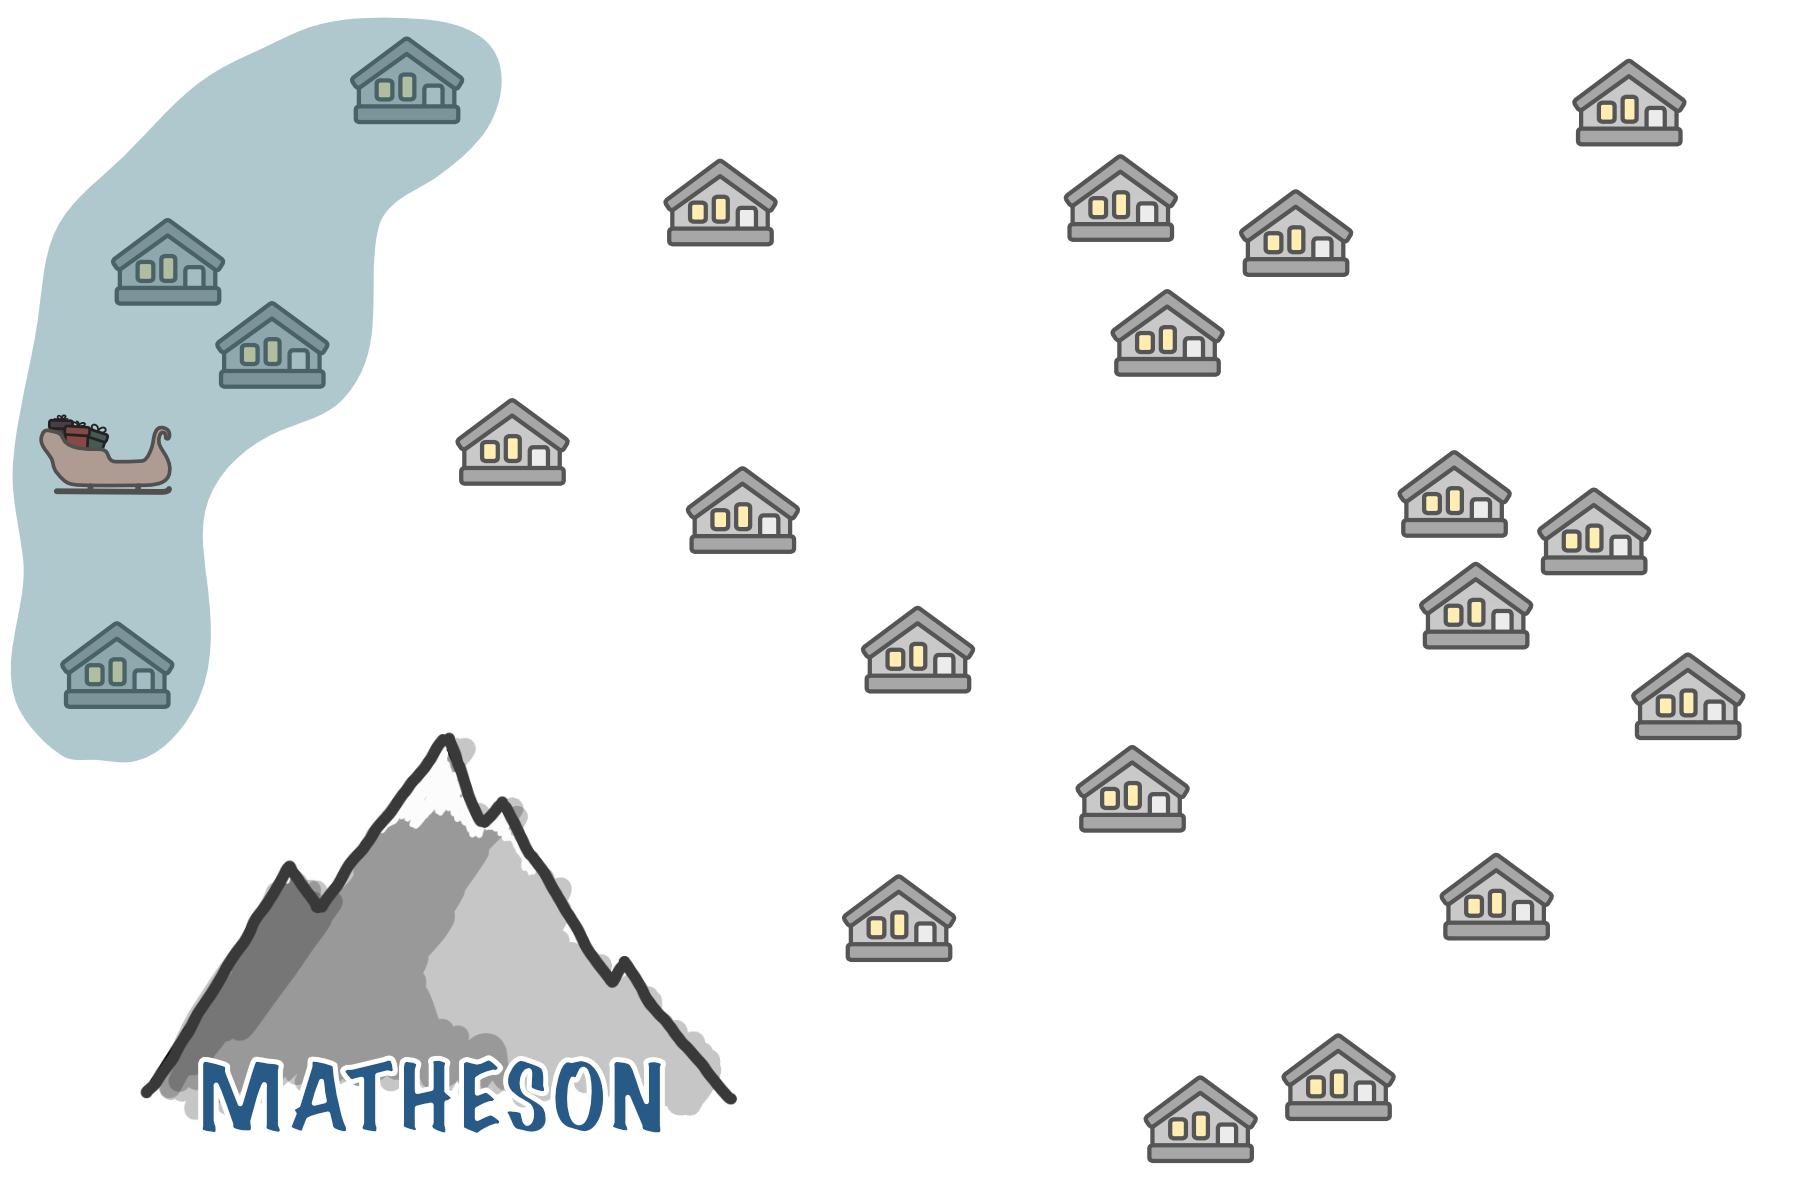
\includegraphics[width=\textwidth]{Images/Matheson/Matheson_03}
\end{frame}

\begin{frame}[fragile]{Motivation}
    \hspace*{-.25em}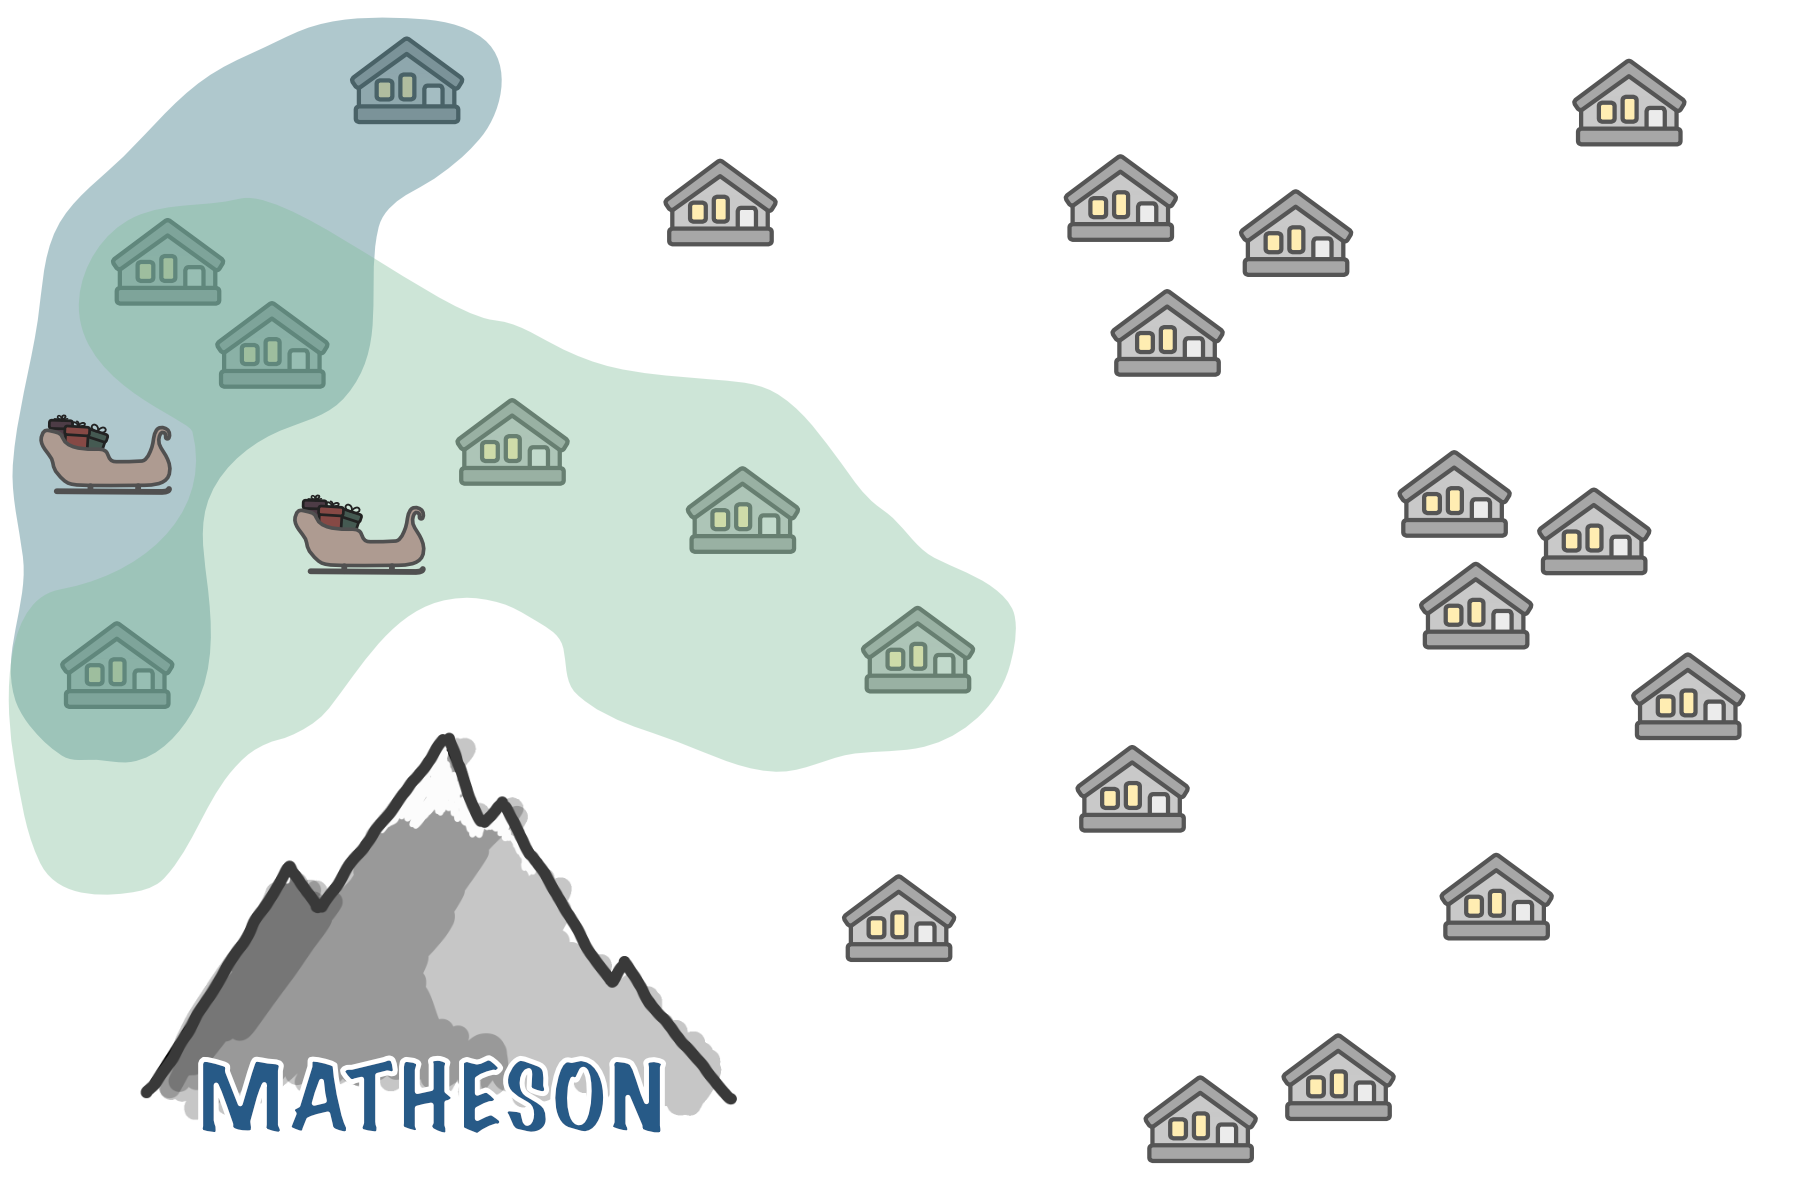
\includegraphics[width=\textwidth]{Images/Matheson/Matheson_04}
\end{frame}

\begin{frame}[fragile]{Motivation}
    \hspace*{-.25em}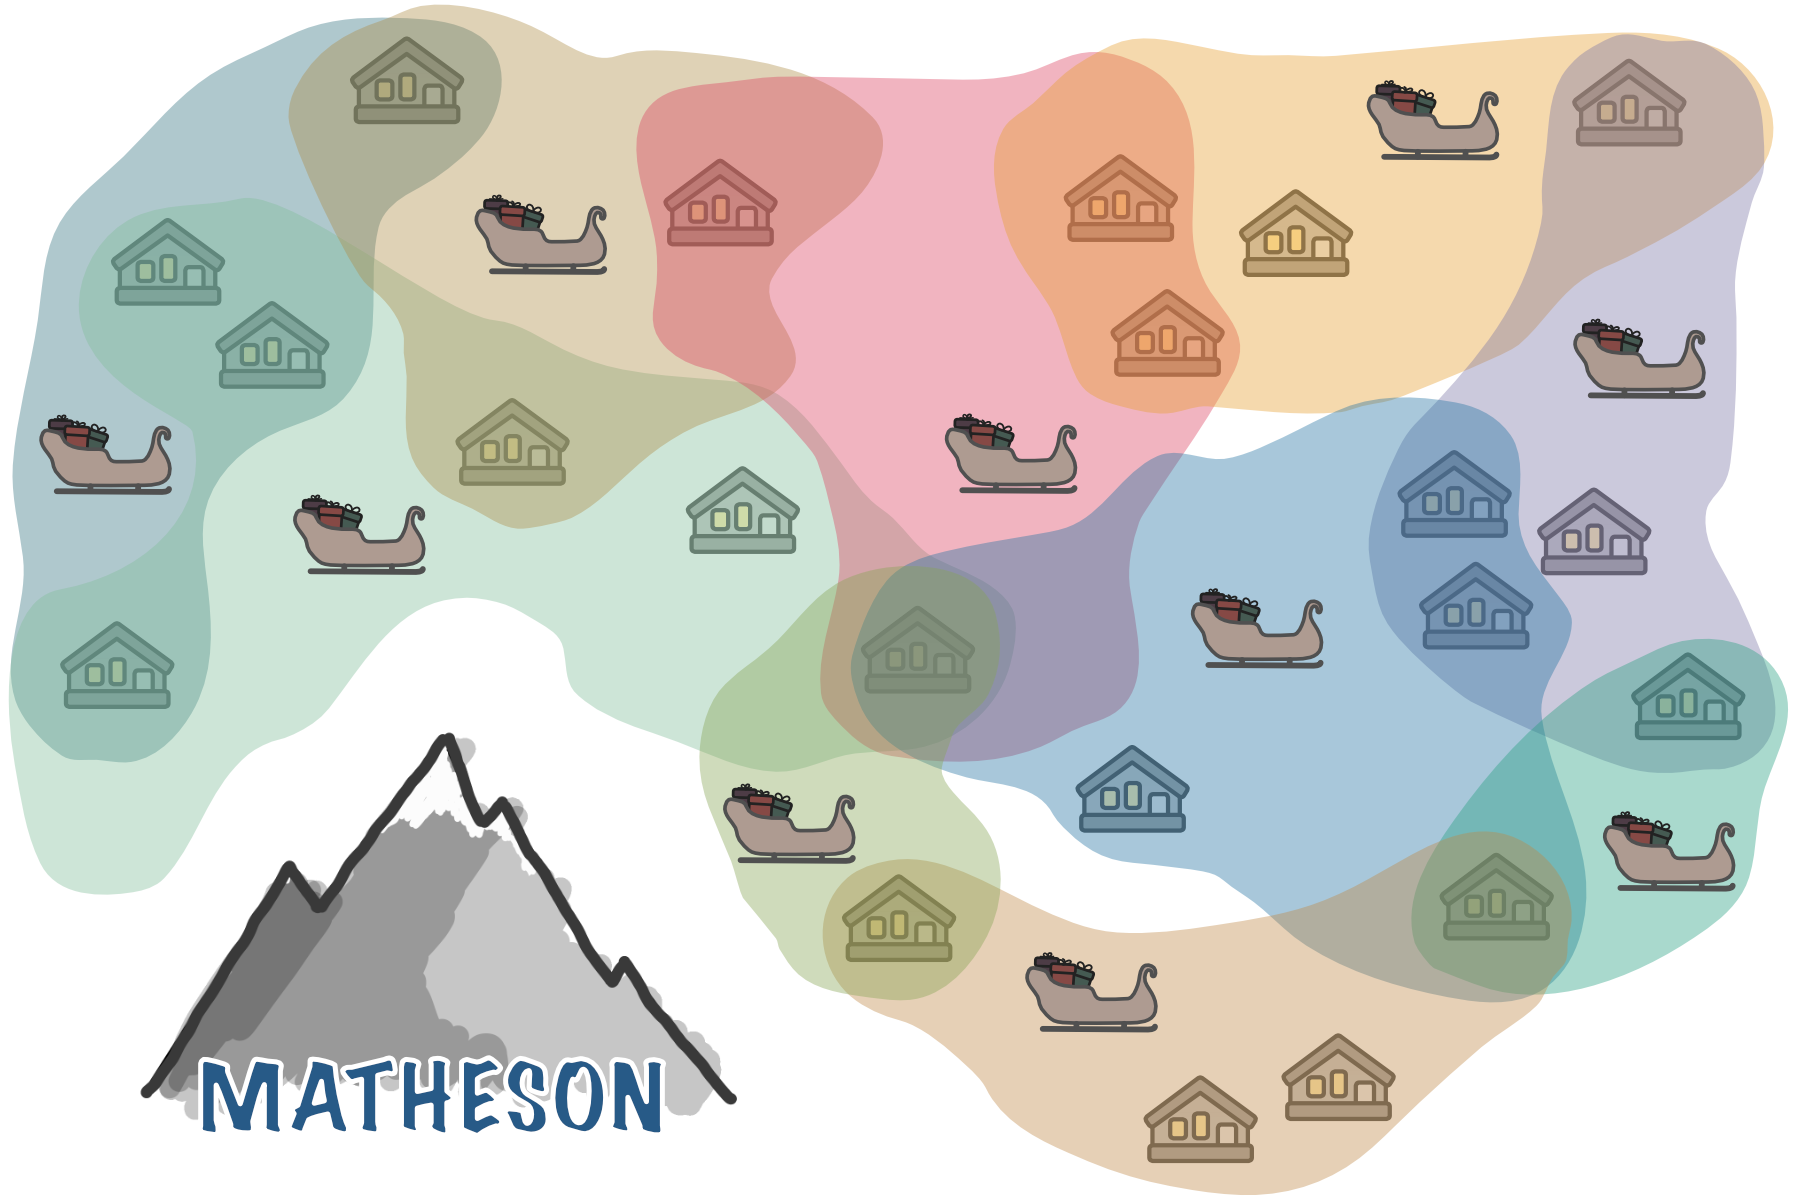
\includegraphics[width=\textwidth]{Images/Matheson/Matheson_05}
\end{frame}

\begin{frame}[fragile]{Motivation}
    \hspace*{-.25em}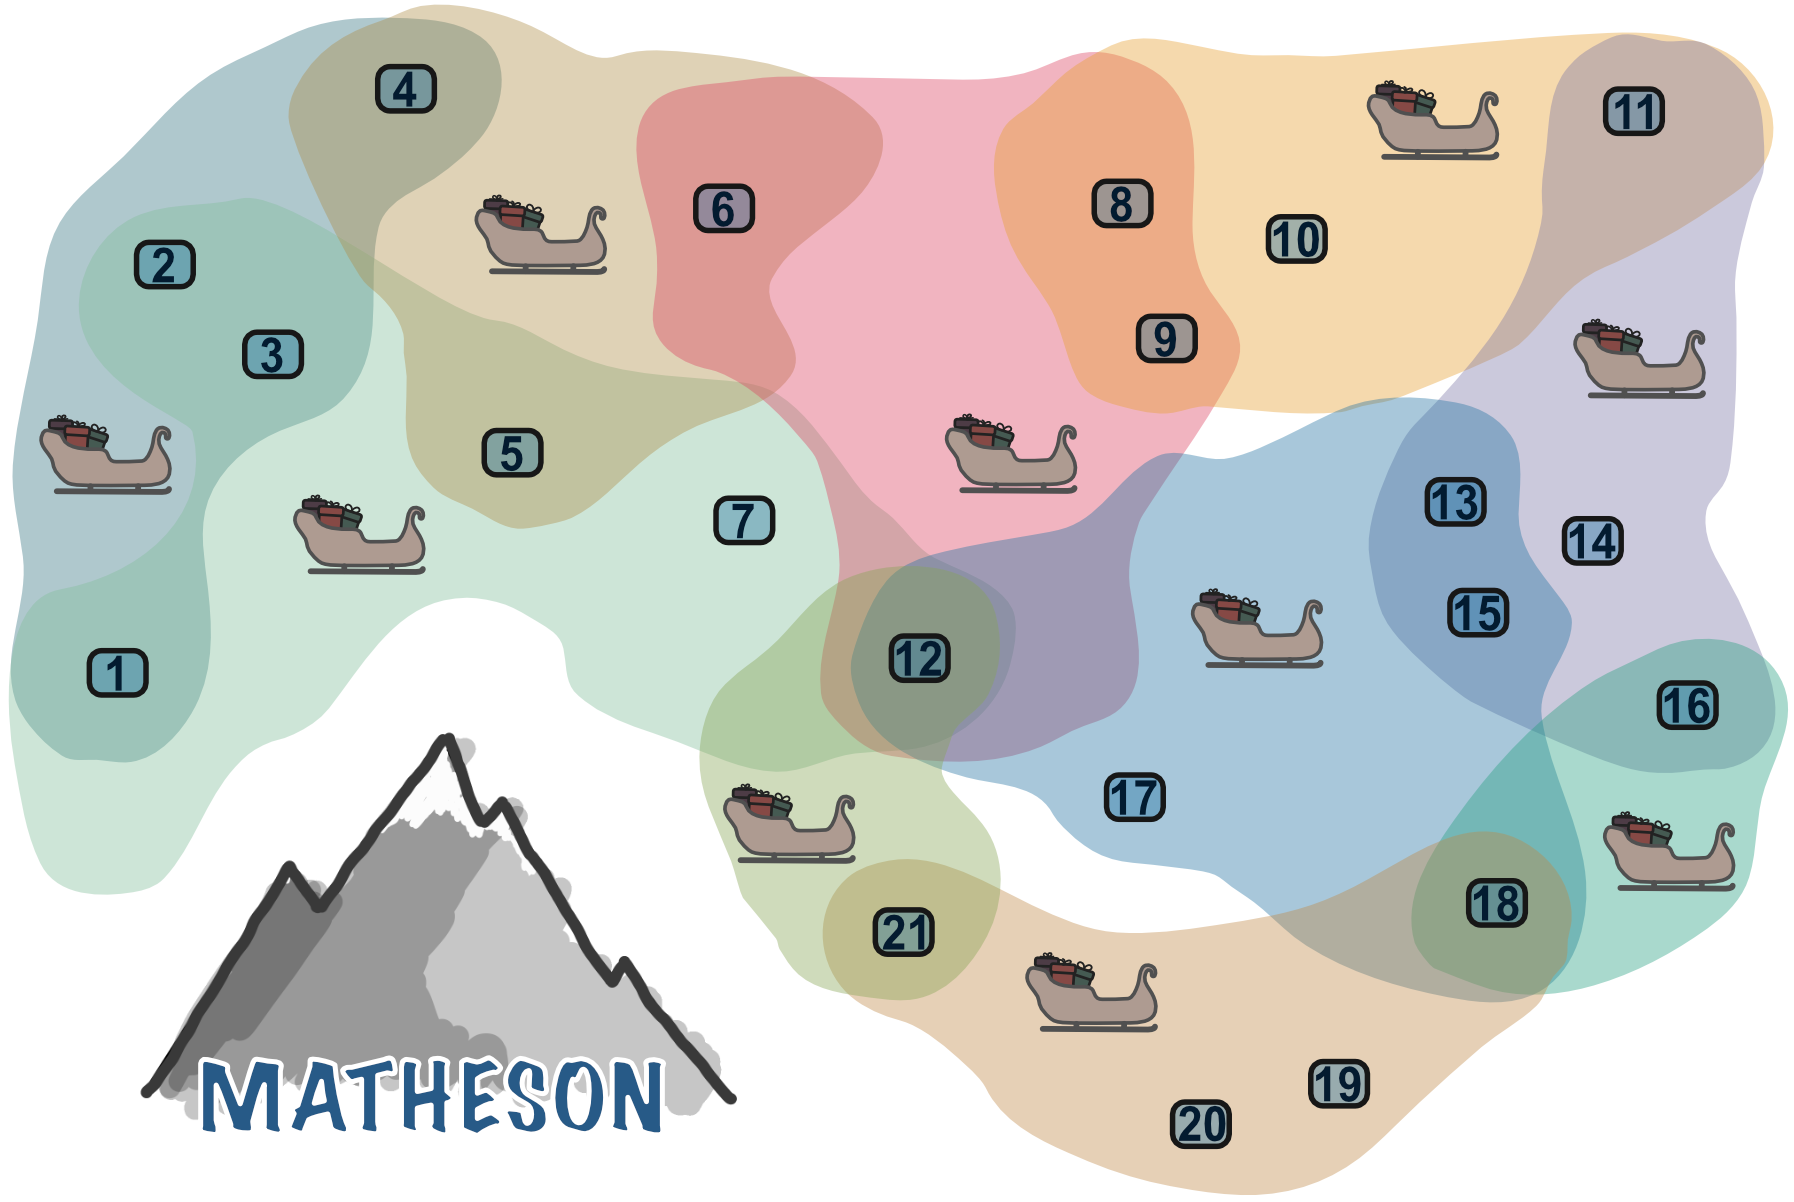
\includegraphics[width=\textwidth]{Images/Matheson/Matheson_06}
\end{frame}

\begin{frame}[fragile]{Motivation}
    \hspace*{-.25em}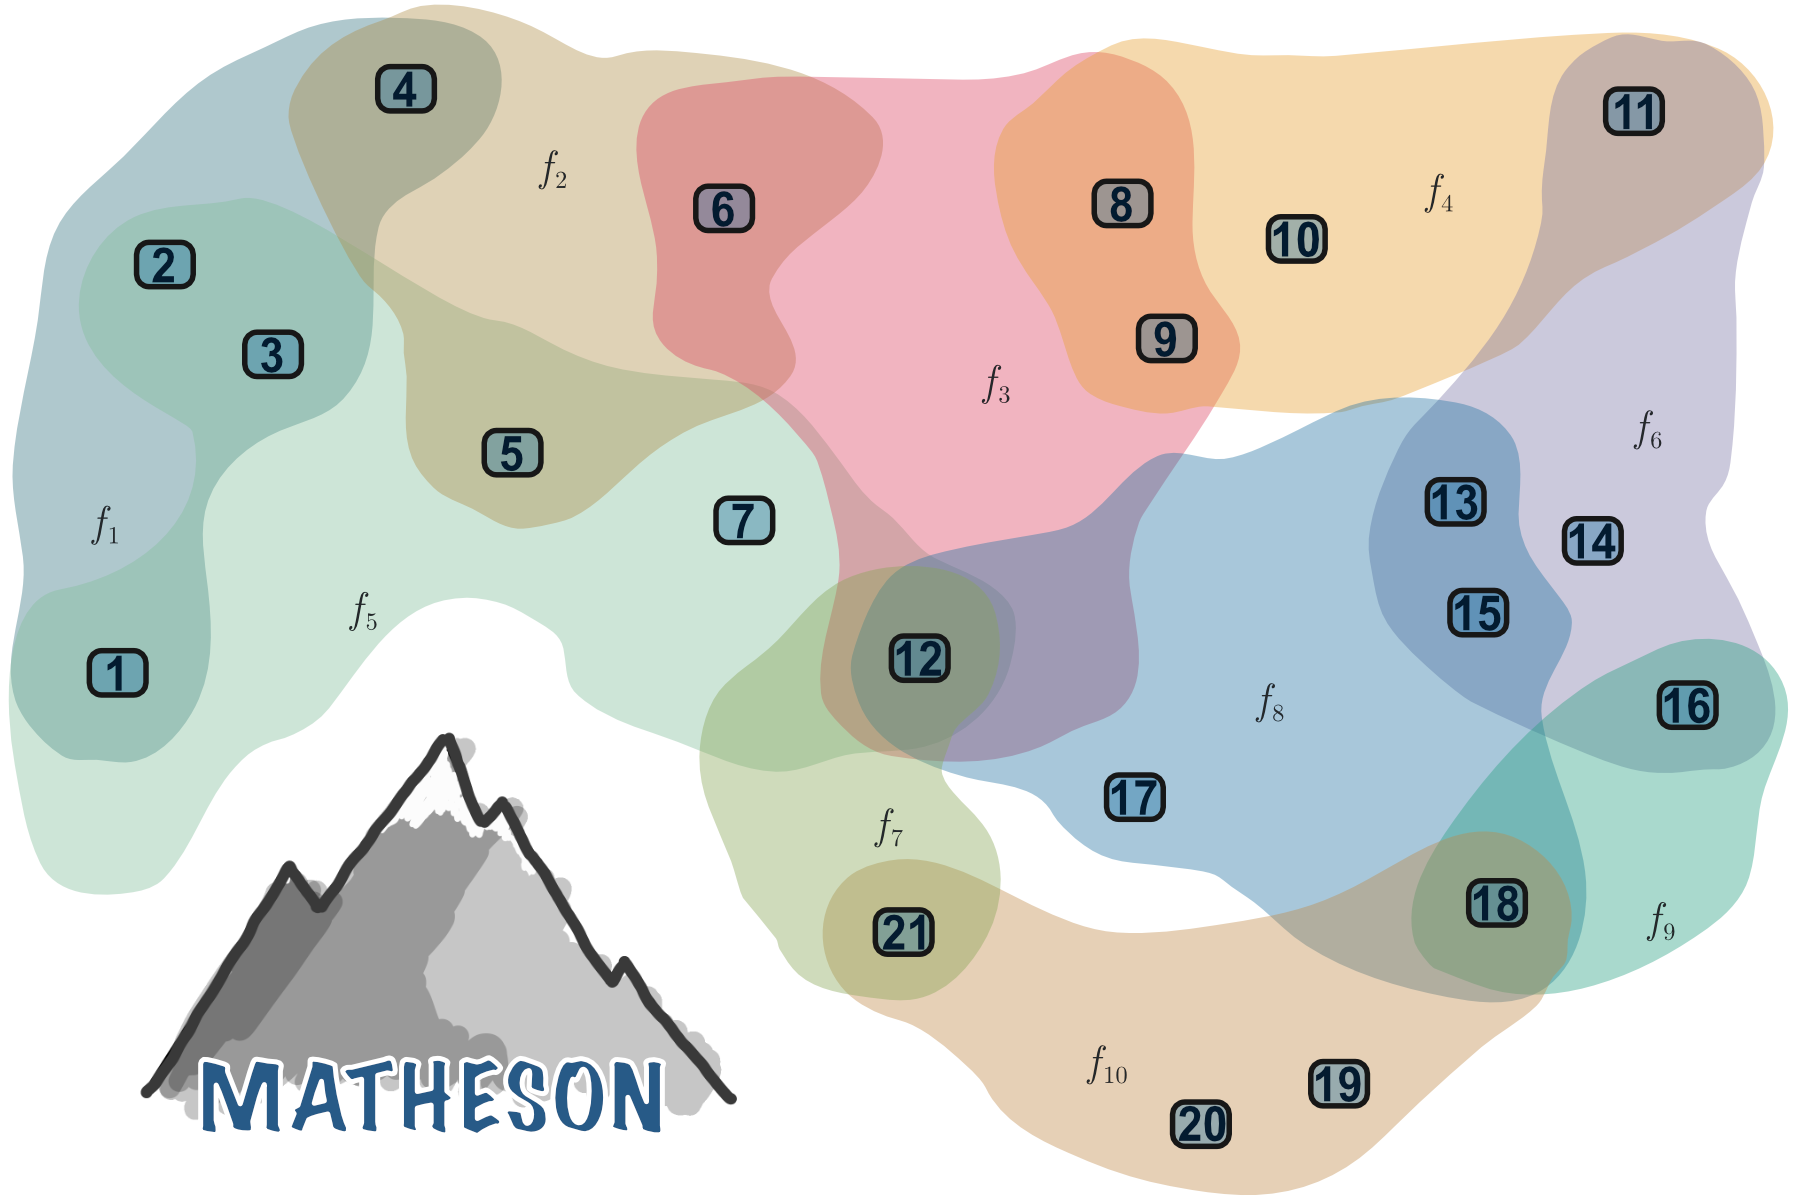
\includegraphics[width=\textwidth]{Images/Matheson/Matheson_07}
\end{frame}

%%%%%%%%%%%%%%%%%%%%%%%%%%%%%%%%%%%%%%%%%%%%%%%%%%%%%%%%%%%%%%%%%%%%%%%%%%%%%%%%%%%
%               The second part of the example starts here.                       %
%%%%%%%%%%%%%%%%%%%%%%%%%%%%%%%%%%%%%%%%%%%%%%%%%%%%%%%%%%%%%%%%%%%%%%%%%%%%%%%%%%%

\begin{frame}[fragile]{Motivation}
    \hspace*{-.25em}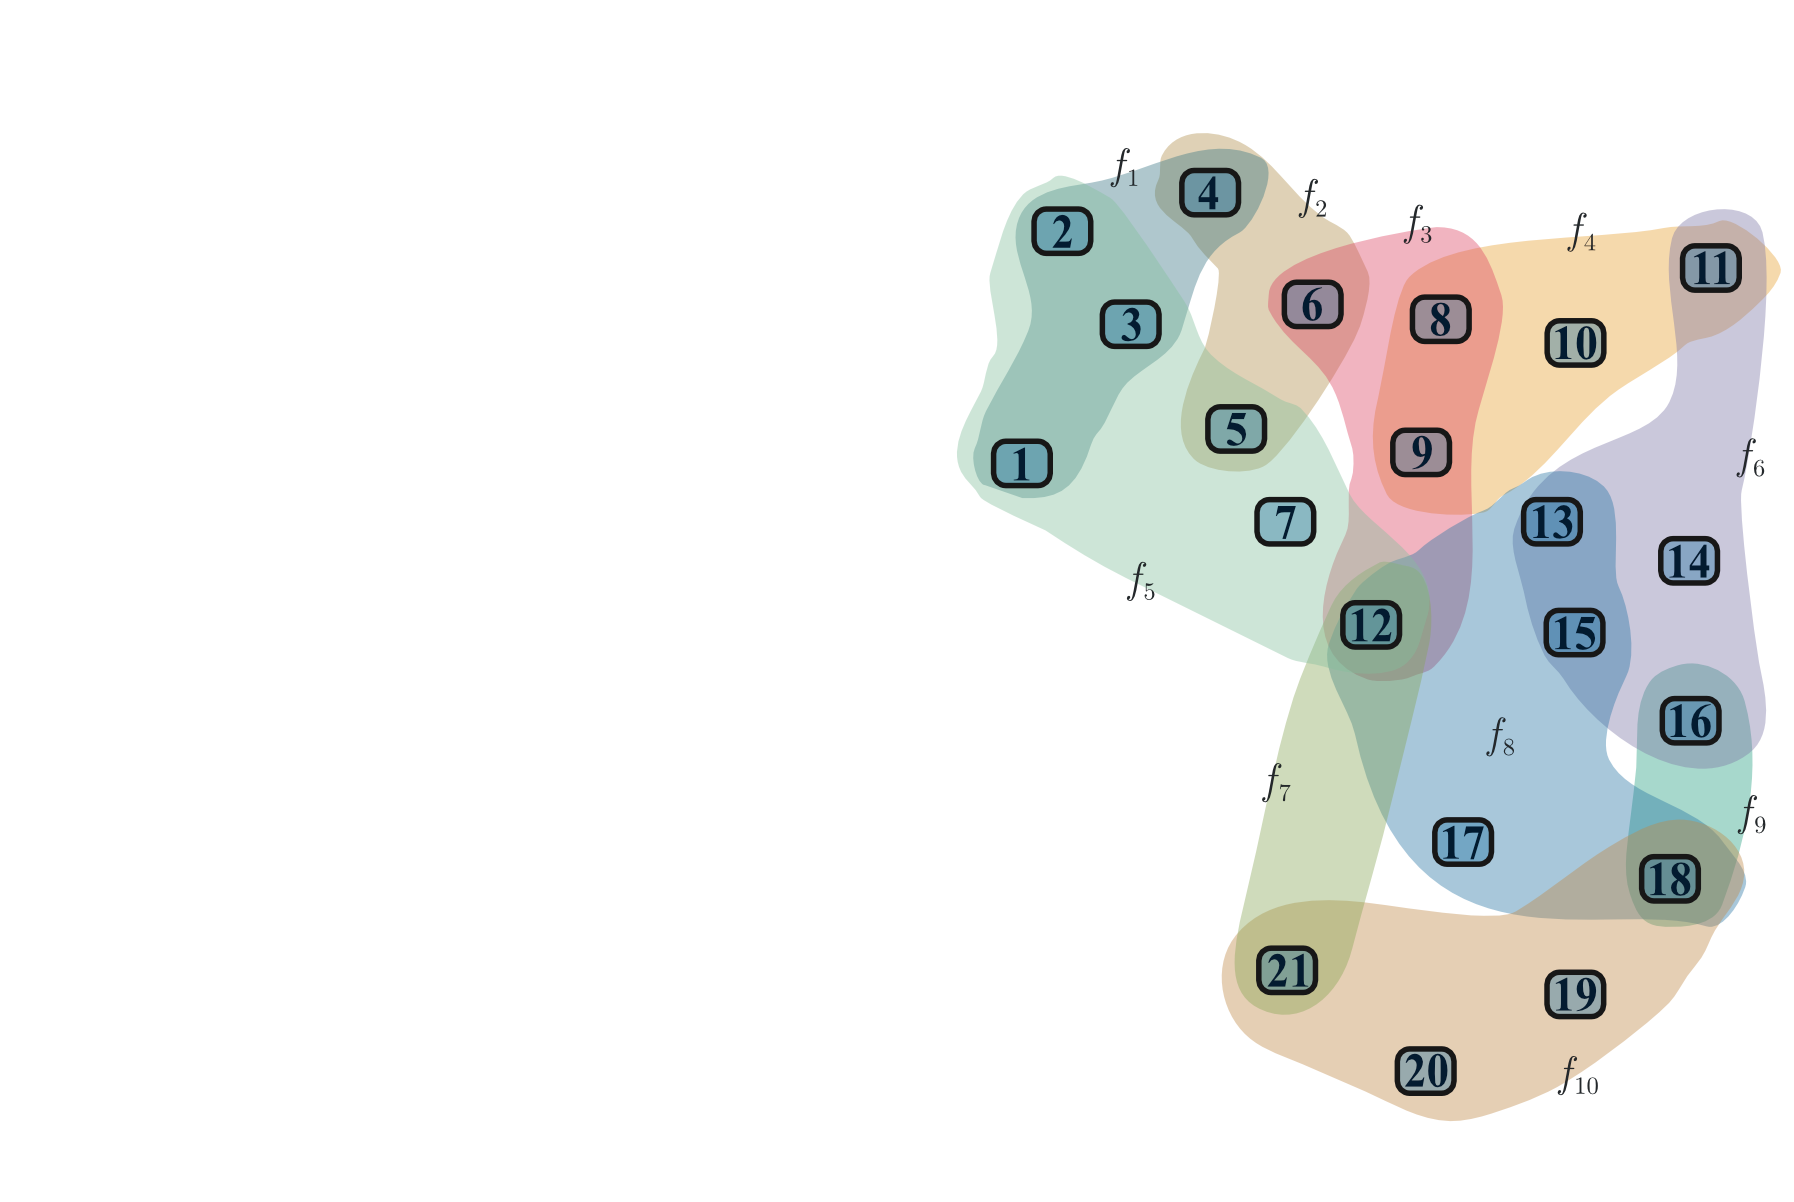
\includegraphics[width=\textwidth]{Images/Matheson/Matheson_10}
\end{frame}

\begin{frame}[fragile]{Motivation}
    \hspace*{-.25em}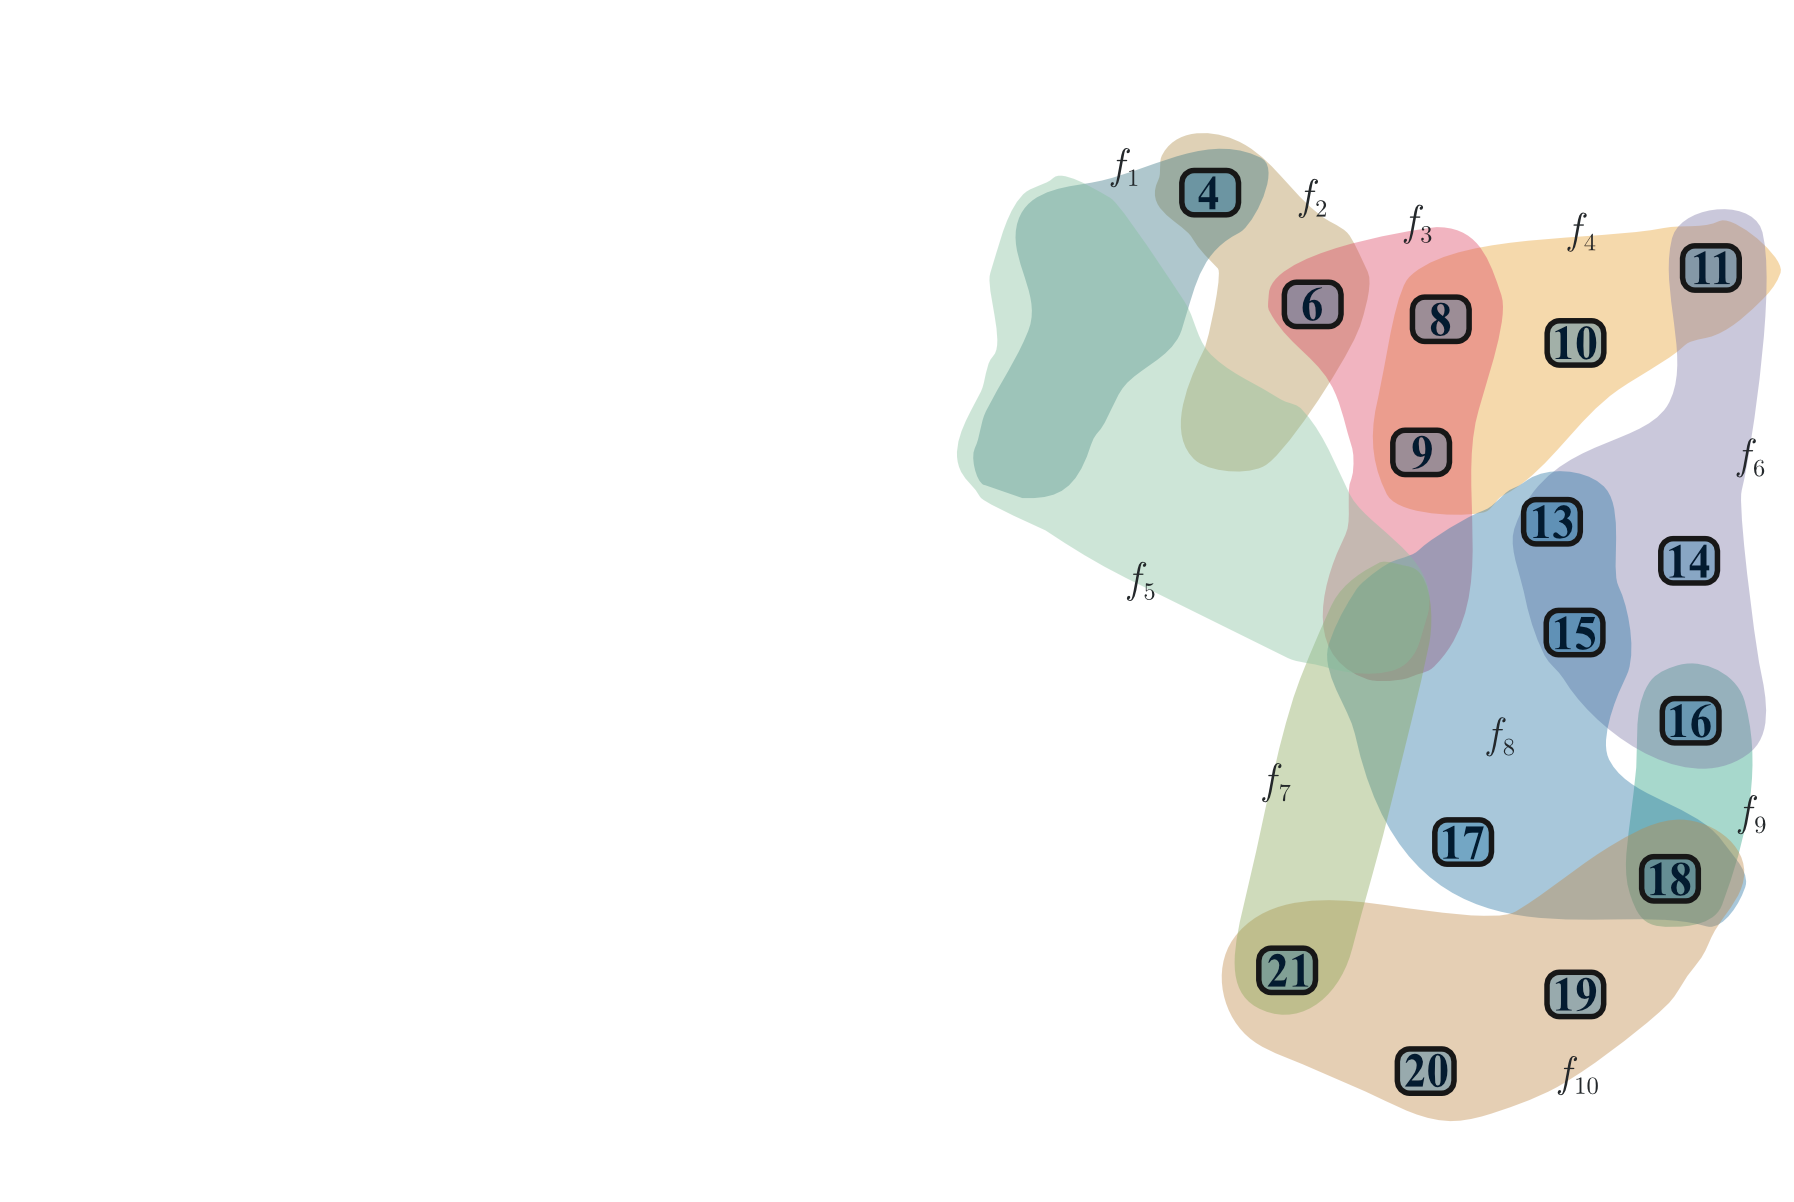
\includegraphics[width=\textwidth]{Images/Matheson/Matheson_11}
\end{frame}

\begin{frame}[fragile]{Motivation}
    \hspace*{-.25em}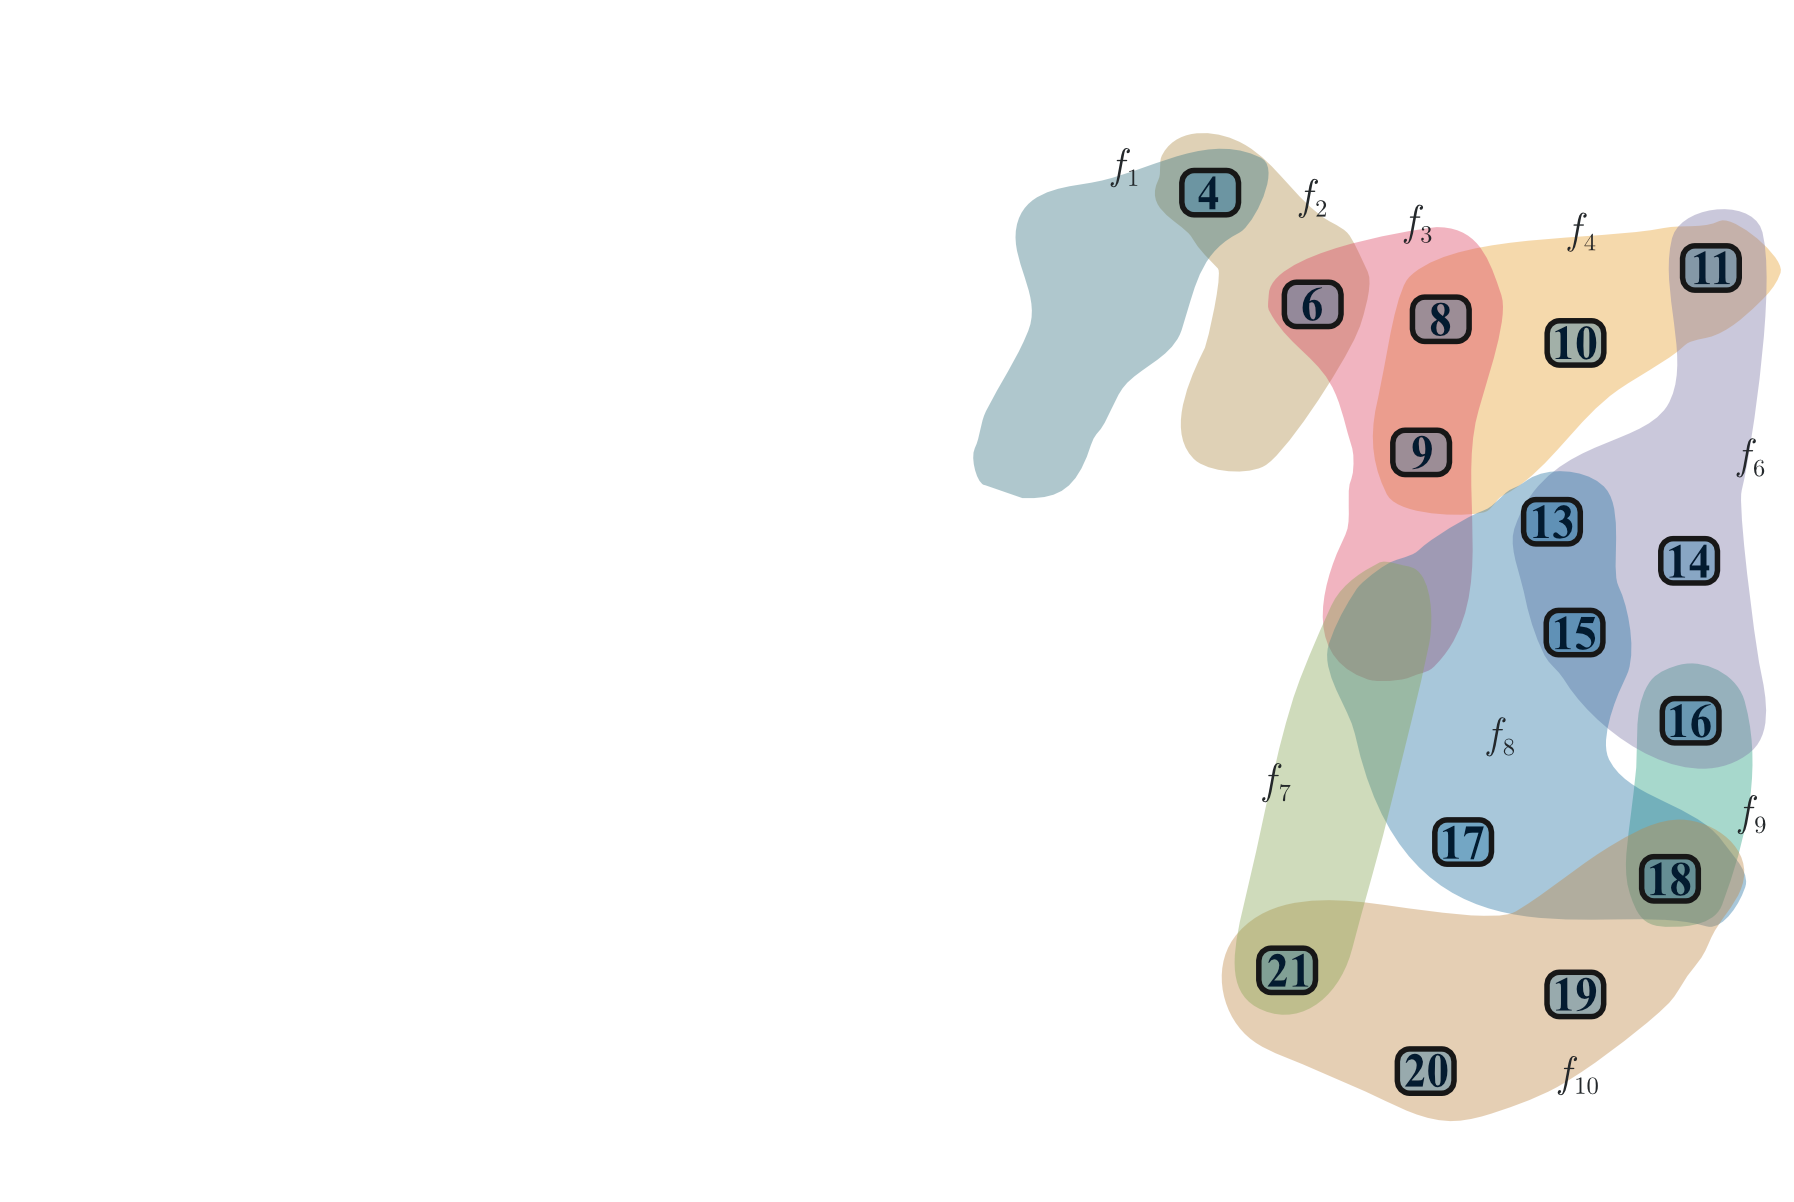
\includegraphics[width=\textwidth]{Images/Matheson/Matheson_12}
\end{frame}

\begin{frame}[fragile]{Motivation}
    \hspace*{-.25em}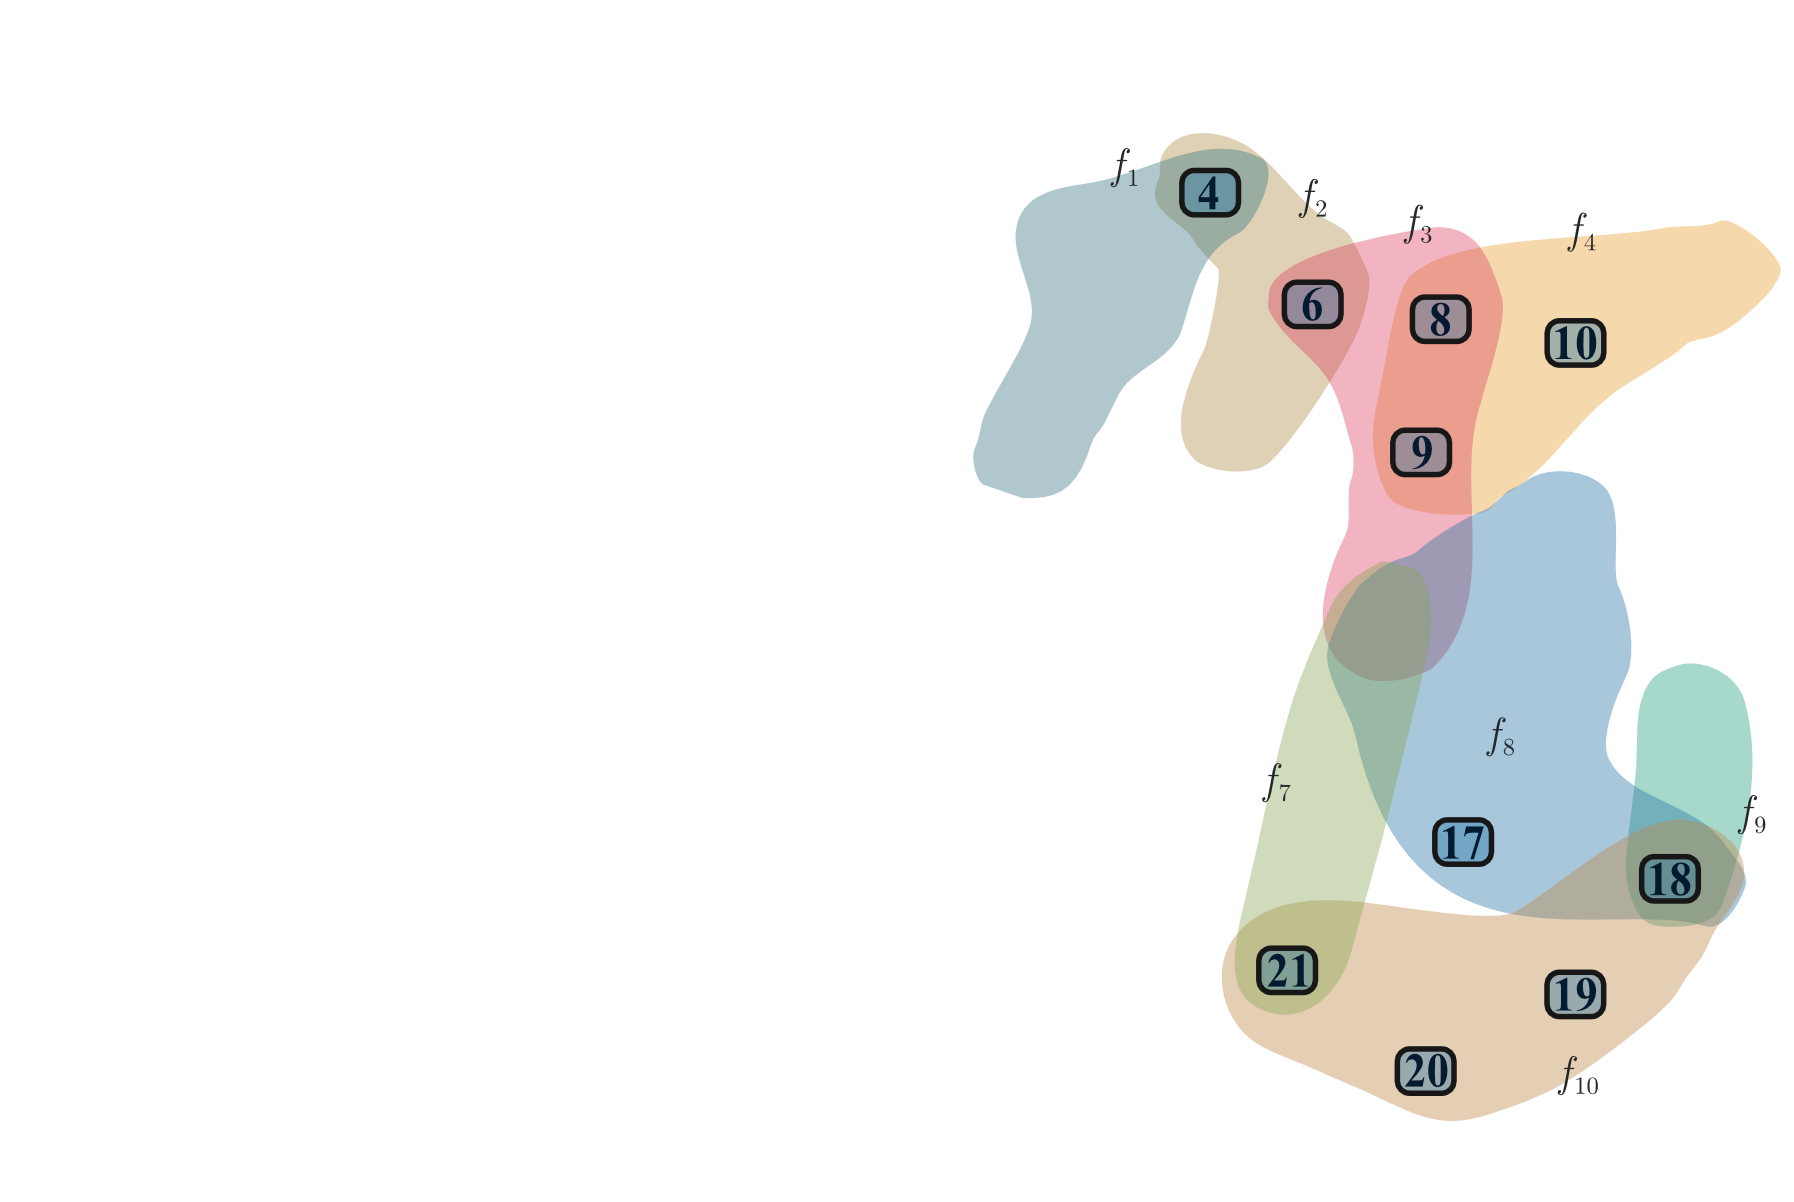
\includegraphics[width=\textwidth]{Images/Matheson/Matheson_13}
\end{frame}

\begin{frame}[fragile]{Motivation}
    \hspace*{-.25em}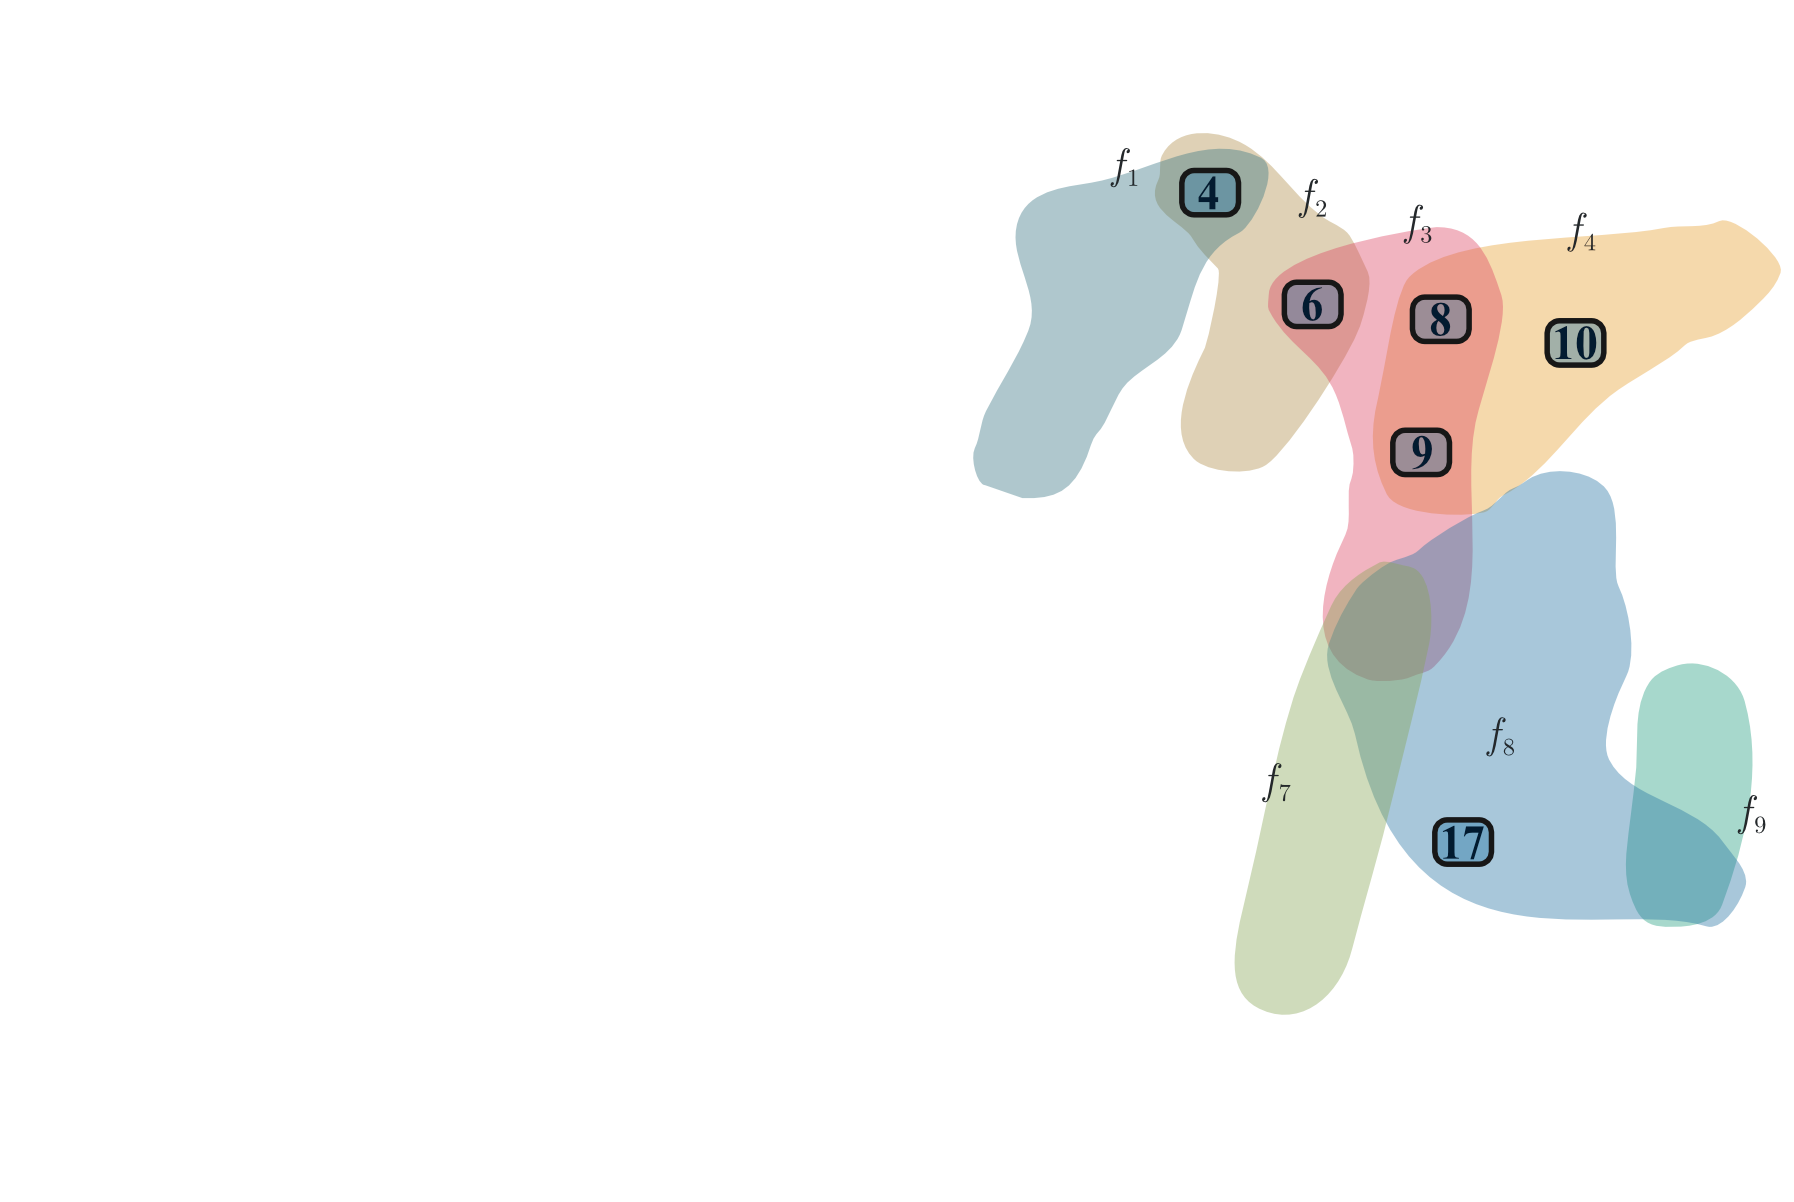
\includegraphics[width=\textwidth]{Images/Matheson/Matheson_14}
\end{frame}

\begin{frame}[fragile]{Motivation}
    \hspace*{-.25em}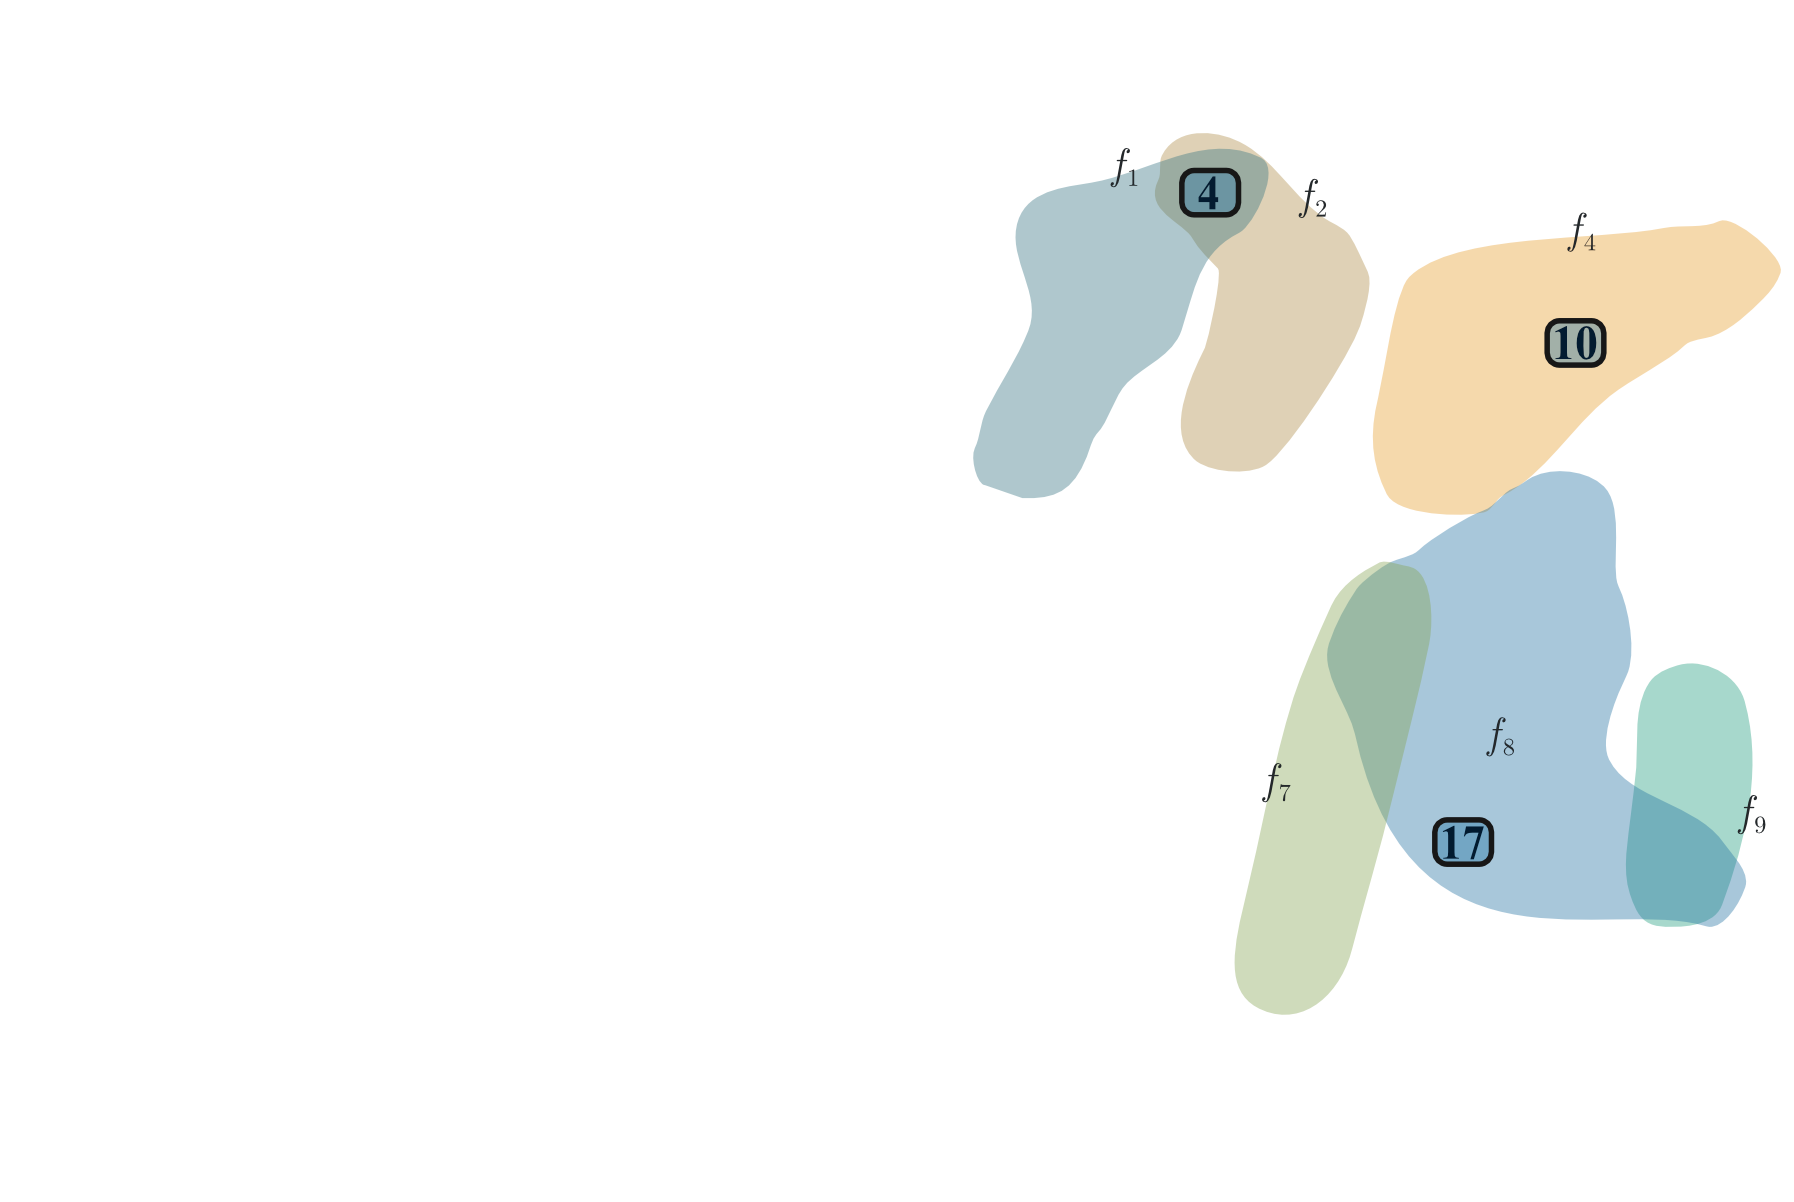
\includegraphics[width=\textwidth]{Images/Matheson/Matheson_15}
\end{frame}

\begin{frame}[fragile]{Motivation}
    \hspace*{-.25em}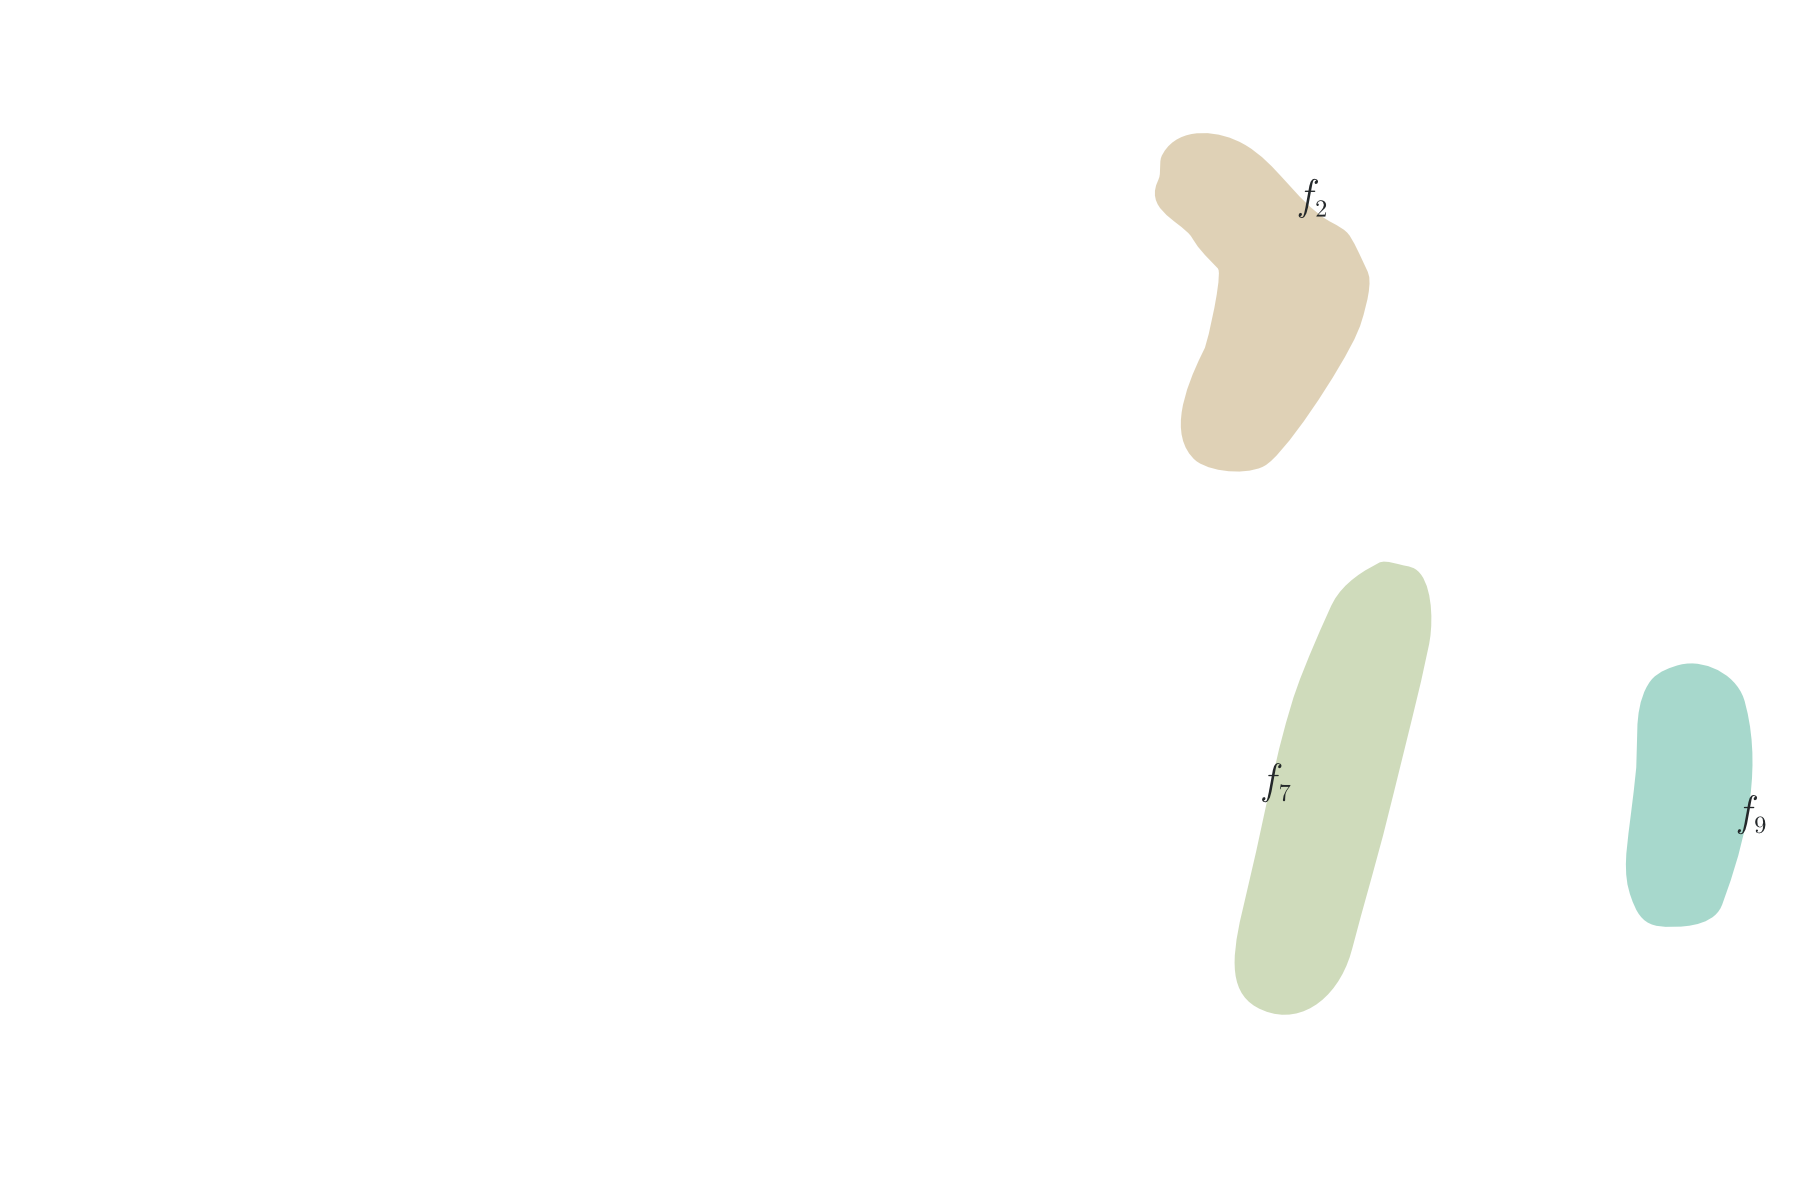
\includegraphics[width=\textwidth]{Images/Matheson/Matheson_16}
\end{frame}



\begin{frame}[fragile]{Lovász-Stein-Theorem}
    \metroset{block=fill}
    \begin{block}{Lovász-Stein Theorem (1974)}
        If each member of $ \mathcal{F} $ has at most $ a $ elements,
        and each point belongs to at least $ v $ of the sets in $ \mathcal{F} $, then
        \[
            Cov(\mathcal{G}) \leq \frac{|\mathcal{F}|}{v}(1 + \ln(a)).
        \]
    \end{block}
\end{frame}

\section{Hashing}

\begin{frame}[fragile]{Hash Functions Motivation}
    How fast can $ x \stackrel{?}{\in} M $ be decided by an algorithm? \pause
    \\
    \vspace{1em}
    Some ideas
    \begin{itemize}
        \item[$ (1) $] For each $ m \in M $ check $ x \stackrel{?}{=} m $.\pause
        \item[$ (2) $] If $ M $ is sortable, all elements can be stored in a binary tree of height $ \log (|M|)$.
        Traverse the tree, checking $ x \stackrel{?}{=} m $ for all visited elements $ m $.\pause
    \end{itemize}
    We get a linear-time algorithm for $ (1) $ and a logarithmic-time algorithm for $ (2) $.\pause
    \\
    \vfill
    \textbf{Question}: How close can we get to constant-time?
\end{frame}


\begin{frame}[fragile]{Hash Functions}
    \textbf{Idea}:
    \vspace{-.75em}
    \begin{itemize}
        \item Use a function $ h : M \to [n] $, \pause
        \item that can be evaluated in $ \mathcal{O}(1) $ time,\pause
        \item to map elements of $ M $ to positions $ 1, \dots, n $. \pause
    \end{itemize}
    \\
    \vfill

    \textbf{Example} ($ h(x) = x \text{ mod } 5 $):
    \begin{columns}[T]
    \begin{column}{.3\textwidth}
        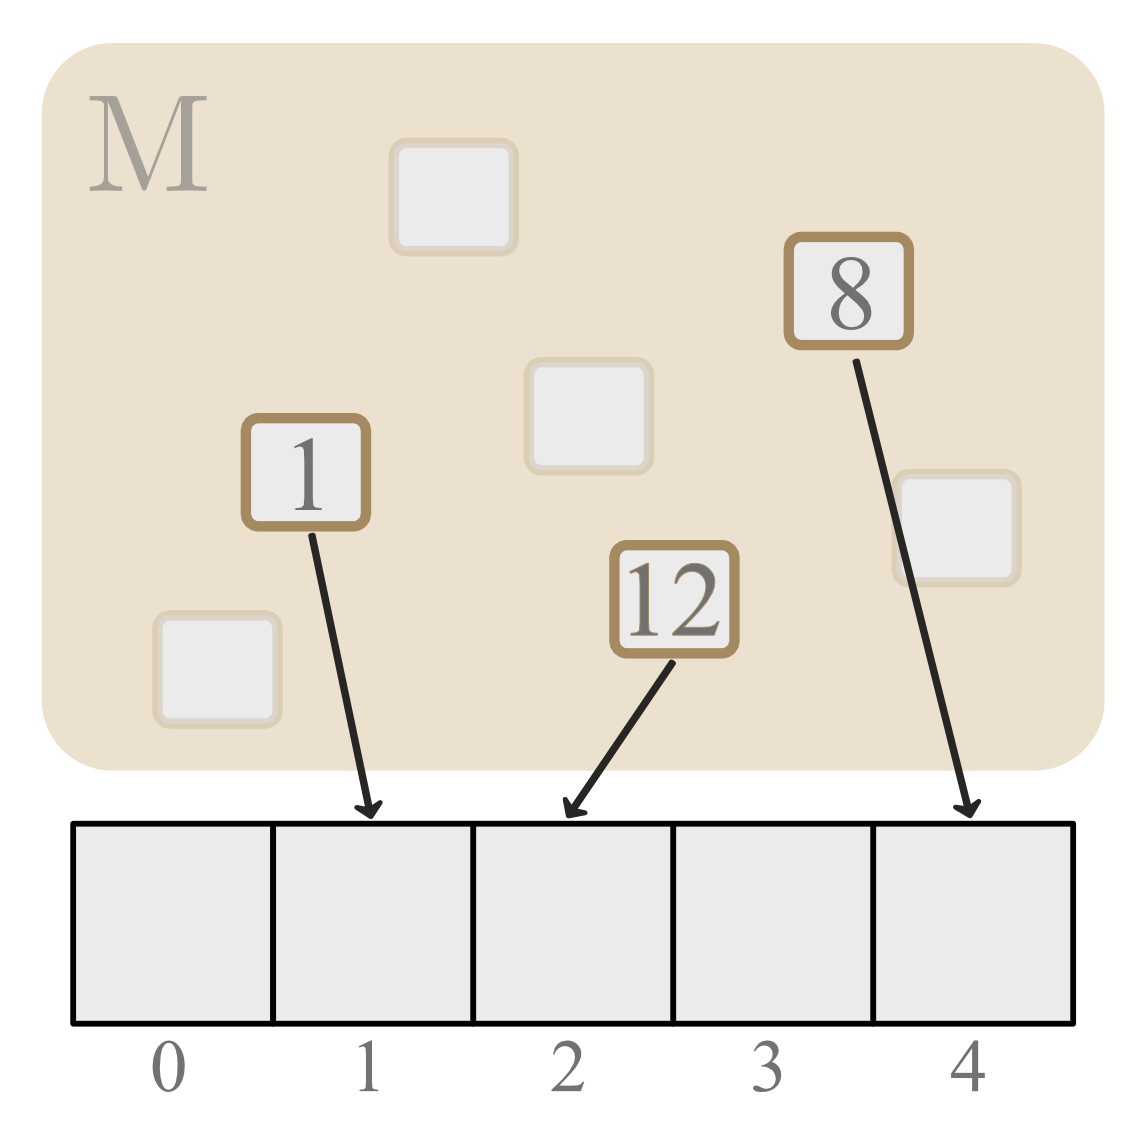
\includegraphics[height=.5\textheight]{Images/Hashing/Hashing_01}
    \end{column}

    \begin{column}{.5\textwidth}
        %\begin{itemize}
        %    \item What happens if two items are mapped to the same position?
        %    \item Time-complexity?
        %\end{itemize}
        %\vspace{3em}
        %$ \to $ Hashing with linear probing on sufficiently large arrays results in \textit{expected constant time}.
    \end{column}
    \end{columns}

    %\textbf{Question}: Can we get constant-time?
\end{frame}

\begin{frame}[fragile]{Hash Functions}
    \textbf{Idea}:
    \vspace{-.75em}
    \begin{itemize}
        \item Use a function $ h : M \to [n] $,
        \item that can be evaluated in $ \mathcal{O}(1) $ time,
        \item to map elements of $ M $ to positions $ 1, \dots, n $.
    \end{itemize}
    \\
    \vfill

    \textbf{Example} ($ h(x) = x \text{ mod } 5 $):
    \begin{columns}[T]
    \begin{column}{.3\textwidth}
        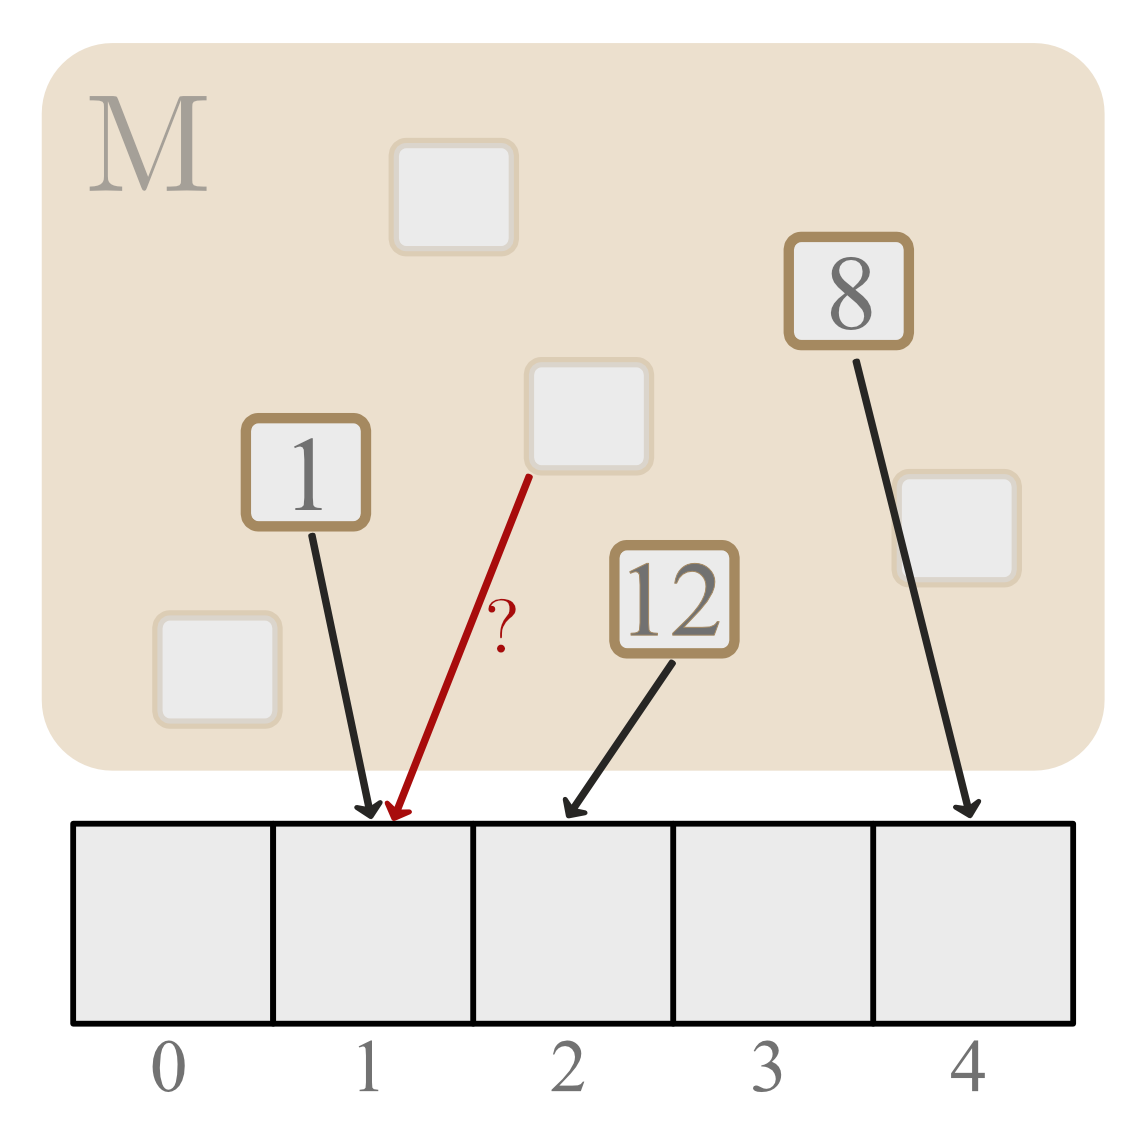
\includegraphics[height=.5\textheight]{Images/Hashing/Hashing_02}
    \end{column}

    \begin{column}{.5\textwidth}
        \begin{itemize}
            \item What happens if two items get mapped to the same position? \pause
            \item Time-complexity? \pause
        \end{itemize}
        \vspace{3em}
        $ \to $ Hashing with linear probing on sufficiently large arrays results in \textit{expected constant time}. \pause
    \end{column}
    \end{columns}

    \textbf{Question}: Can we get to constant-time?
\end{frame}


\begin{frame}[fragile]{Perfect Hash Functions}
    Let $ \mathcal{F} $ be a family of $ N $-many functions $ f : X \to Y $, where
    $ |X| = n $, $ |Y| = m $.
    
    \textbf{Definition.} The family $ \mathcal{F} $ is a perfect hashing family (PHF), if
    $ \forall C \subseteq X, |C| = w: \exists f \in \mathcal{F}: \restr{f}{C} $ is injective.

    \vfill

    \metroset{block=fill}
    \begin{block}{Theorem 2 (2011)}
        There exists a perfect hashing family with
        \[
            N \leq \frac{n^w}{w!{n \choose w}}\bigg(1 + \ln{m \choose w}\bigg).
        \]
    \end{block}
\end{frame}




\begin{frame}[fragile]{References}
    \nocite{*}
    \bibliographystyle{alpha}
    \bibliography{bibliography}
\end{frame}

\end{document}
